%%%% ijcai22.tex

\typeout{IJCAI--22 Instructions for Authors}

% These are the instructions for authors for IJCAI-22.

\documentclass{article}
\pdfpagewidth=8.5in
\pdfpageheight=11in
% The file ijcai22.sty is NOT the same than previous years'
\usepackage{ijcai22}

% Use the postscript times font!
\usepackage{times}
\usepackage{soul}
\usepackage{url}
\usepackage[hidelinks]{hyperref}
\usepackage[utf8]{inputenc}
\usepackage[small]{caption}
\usepackage{graphicx}
\usepackage{amsmath}
\usepackage{amsthm}
\usepackage{amssymb,amsfonts}
\usepackage{booktabs}
\usepackage{algorithm}
\usepackage{algorithmic}
\usepackage{color}
\usepackage{subcaption}
\usepackage{enumitem}
\usepackage{pifont}
\usepackage{mathtools}
\usepackage{arydshln}
\usepackage{multirow}
% \usepackage{subfigure}
% \usepackage{array}
\urlstyle{same}

\newcommand{\modelParamter}{\omega}
\newcommand{\horizon}{T_{H}}
\newcommand{\datapoint}{x}
\newcommand{\condition}{z_{E}}
\newcommand{\state}{s}
\newcommand{\observation}{o}
\newcommand{\action}{a}
\newcommand{\transition}{t}
\newcommand{\reward}{r}
\newcommand{\agentIndex}{k}
\newcommand{\gameIndex}{j}
\newcommand{\quantielIndex}{i}
\newcommand{\dataset}{\mathcal{D}}
\newcommand{\expect}{\mathbb{E}}
\newcommand{\feature}{e}
\newcommand{\confidence}{c}
\newcommand{\error}{\epsilon}
\newcommand{\impact}{\phi}
\newcommand{\playerId}{l}
\newcommand{\constant}{C}
\newcommand{\splitnum}{m}
\newcommand{\sys}{RiGIM}
\newcommand{\bin}{B}
\newcommand{\goal}{g}
\newcommand{\system}{\sys\;}
\newtheorem{example}{Example}
\newtheorem{proposition}{Proposition}
\DeclareMathOperator*{\argmax}{argmax}


%PDF Info Is REQUIRED.
\pdfinfo{
/TemplateVersion (IJCAI.2022.0)
}

% \title{Risk-Sensitive Evaluation for Ice Hockey Player with \\ Distributional Reinforcement Learning }

\title{Data-Driven Reinforcement Learning for \\Risk-Sensitive Player Evaluation in Ice Hockey}

% Single author syntax
\author{
}


\begin{document}

\maketitle

\begin{abstract}
A major task of sports analytics is player evaluation. Previous methods commonly measured the impact of players' actions on desirable outcomes (e.g., goals or winning) without considering the risk induced by stochastic game dynamics.  In this paper, we design a data-driven Reinforcement Learning (RL) framework to learn a risk-sensitive player evaluation metric from spatial-temporal game context. To embed the risk of a player’s movements into the distribution of action-values, we model their 1) {\it aleatoric uncertainty}, which represents the intrinsic stochasticity in a sports game, and 2) {\it epistemic uncertainty}, which is due to a model's insufficient knowledge regarding Out-of-Distribution (OoD) samples. We demonstrate how a distributional Bellman operator and a feature-space density model can capture both uncertainties. Based on such uncertainty estimation, we propose a Risk-sensitive Game Impact Metric (RiGIM) that measures players' performance over a season by conditioning on a specific confidence level. Empirical evaluation, based on over 4M play-by-play ice hockey events, shows that RiGIM correlates highly with standard success measures and is consistently sensitive to different confidence levels.
\end{abstract}

\section{Introduction}

The advancement of player tracking and object detection systems enables data-driven analytics for professional sports players. A common approach to evaluating the contribution of players is to quantify their action impacts.  Previous performance metrics~\cite{Routley2015Markov,Liu2018DRL,Decroos2019Actions,Luo2020IRL} computed the expected impact of an action on scoring or winning a game. However, actions with significantly different impact distributions can have the same expectations. As a result, the expectation-based metrics cannot differentiate the risk-seeking actions from the risk-averse ones. How to distinguish these actions and assign proper credits to the players remains a fundamental challenge in sports analytics.

An important step toward a risk-sensitive evaluation metric is to model the distributions of action values. To achieve this, distributional RL~\cite{bdr2022} predicts the supporting quantiles of action-value distributions. Previous distributional RL methods~\cite{bellemare2017distributional,Dabney2018DistributionalRL,Mavrin2019DistributionalRL} mainly studied virtual environments with deterministic transitions (e.g., Atari), whereas ice hockey games are real environments with stochastic game dynamics and spatial-temporal context features. Moreover, player evaluation, as a data-driven task, requires off-line learning from a fixed dataset without exploration. The learned values must handle the distribution shift experienced at test time.

To mitigate the impact of distribution shift, Offline RL algorithms~\cite{Levine2020OfflineRL} typically strive for conservative policies that discourage visits to Out-of-Distribution (OoD) states by assigning them penalties. However, this approach cannot be scaled to player evaluation since 1) we do not control players, but use RL as an analytical tool to evaluate observed actions in professional games, and 2) penalizing actions in OoD states distorts the evaluation.
%These conservative policies, however, cannot be applied to player evaluation, where RL acts as an analytic tool for evaluating players' movements in the dataset instead of controlling agents.


\begin{figure}
    \centering
    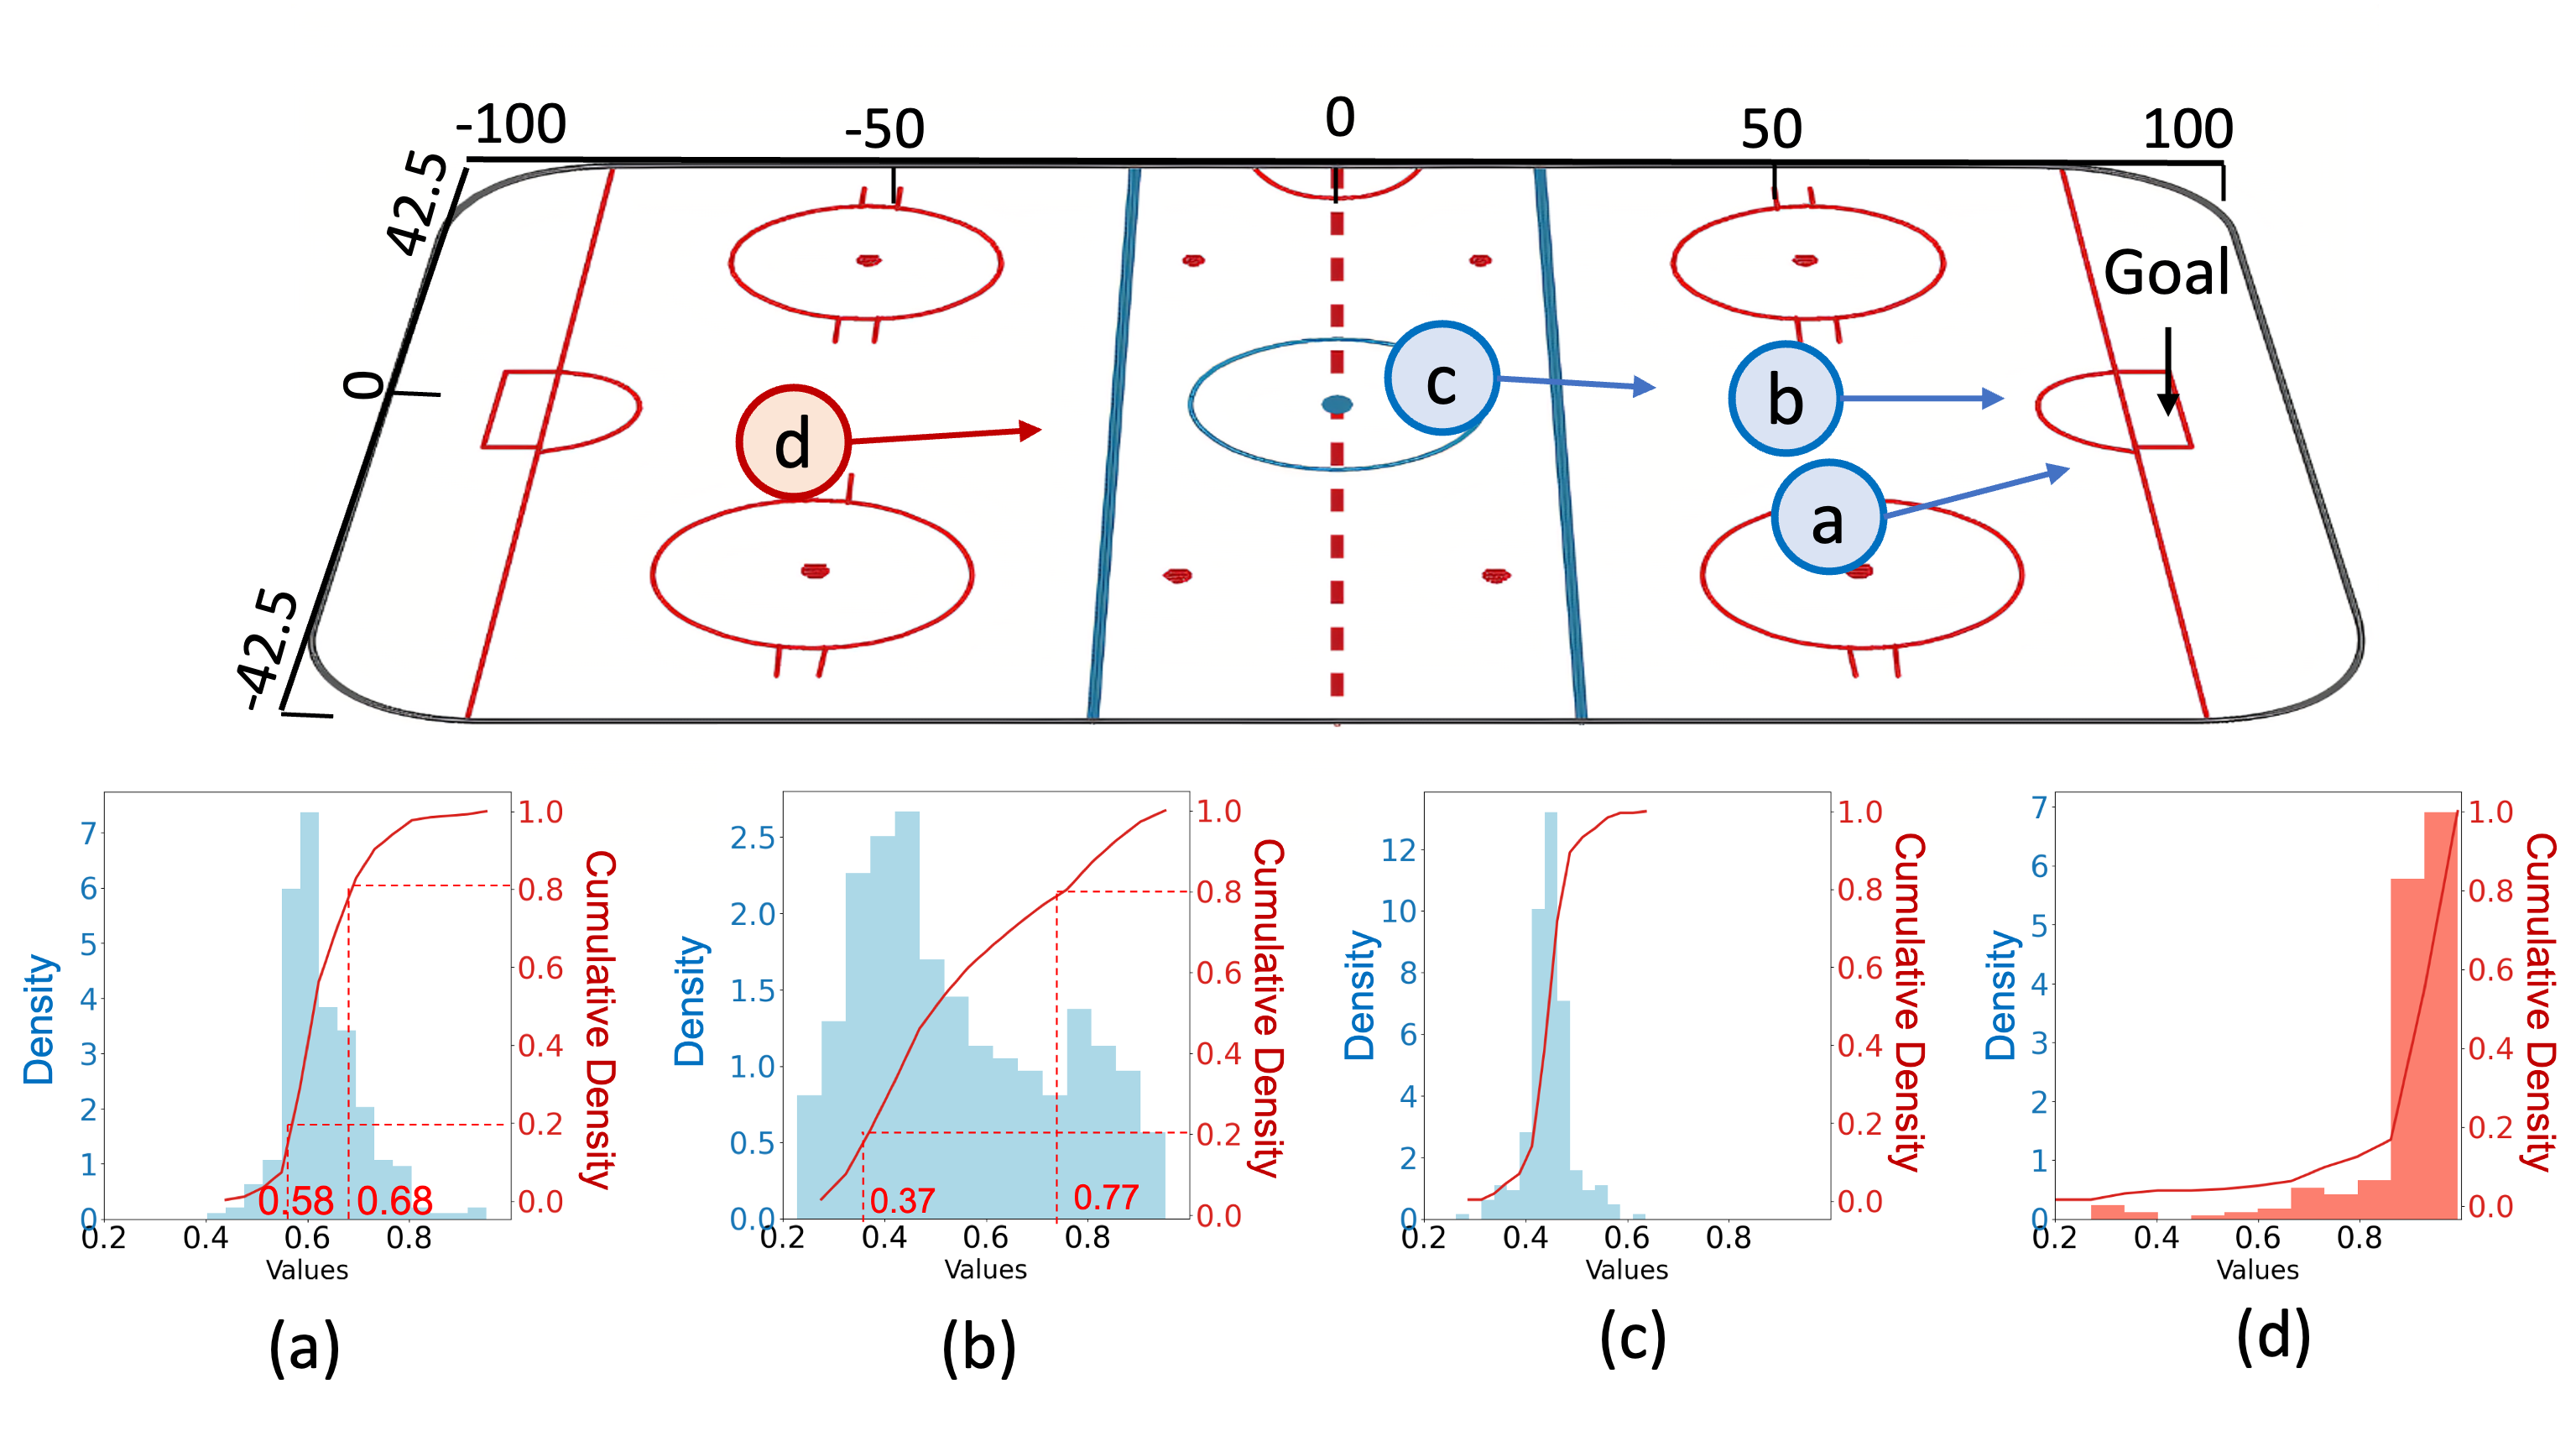
\includegraphics[scale=0.15]{figures/ice-hockey-rink-marked.png}
    % \begin{minipage}{0.5\textwidth}
    % \centering
    % 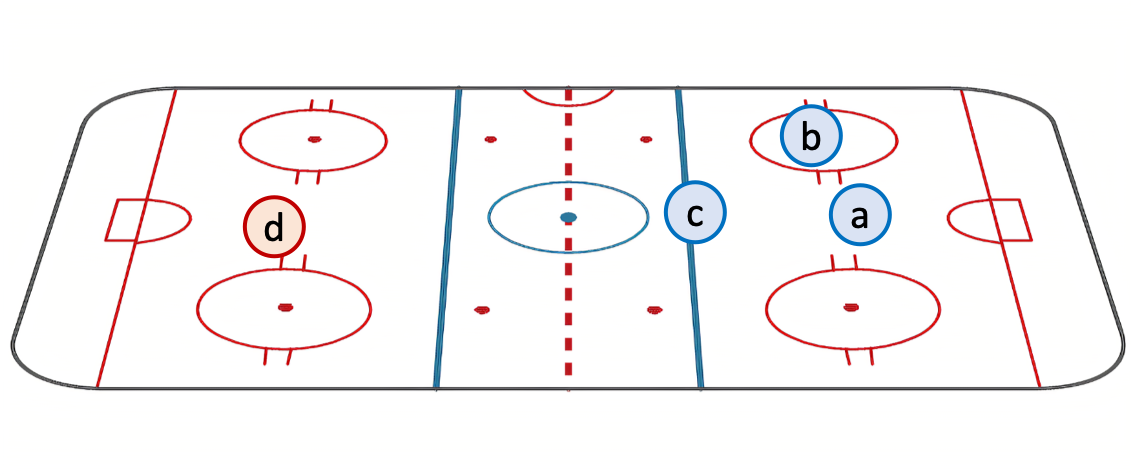
\includegraphics[scale=0.35]{figures/ice-hockey-view-marked.png}
    % \vspace{-0.15in}
    % \end{minipage}
    % \begin{minipage}{0.12\textwidth}
    % \centering
    % 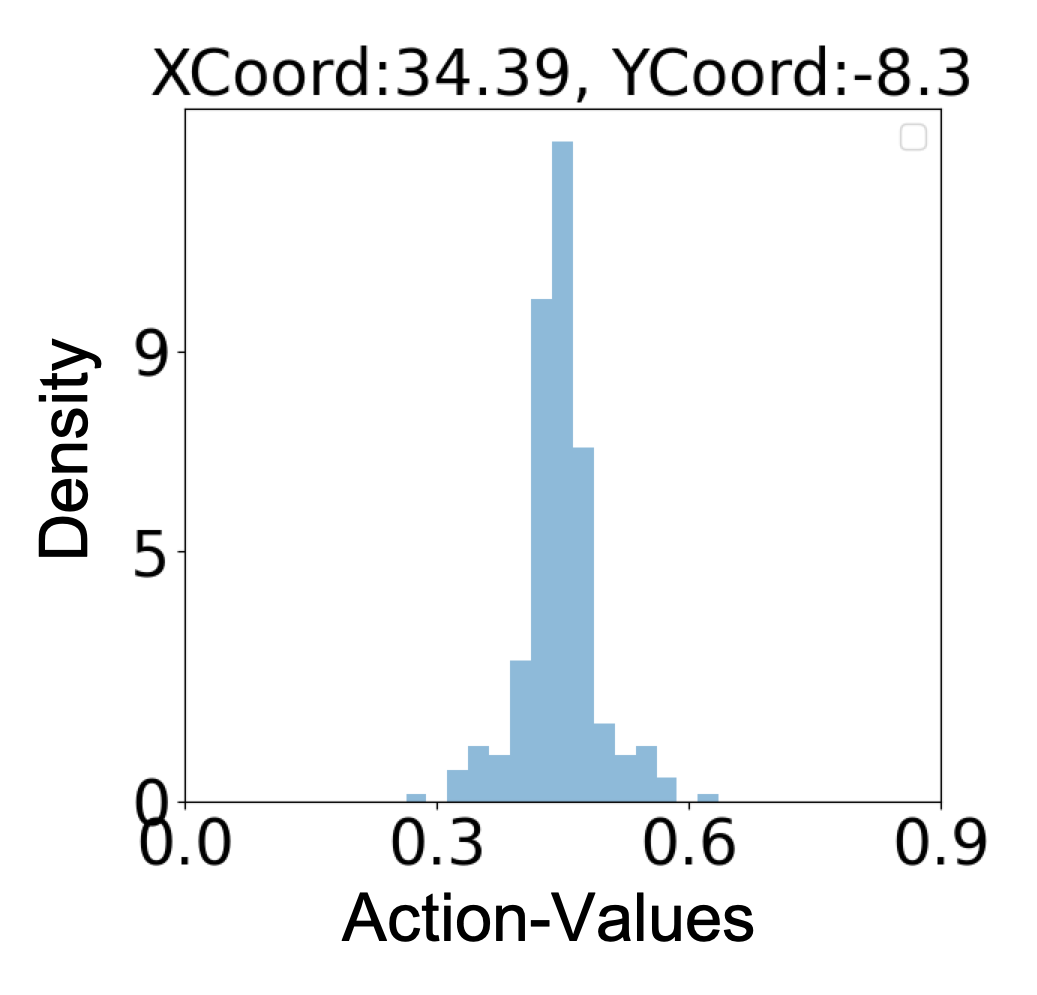
\includegraphics[scale=0.13]{figures/distribution_idx_2_XCoord_34.39_YCoord_-8.3-marked.png}
    % \end{minipage}\hfill
    % \begin{minipage}{0.12\textwidth}
    % 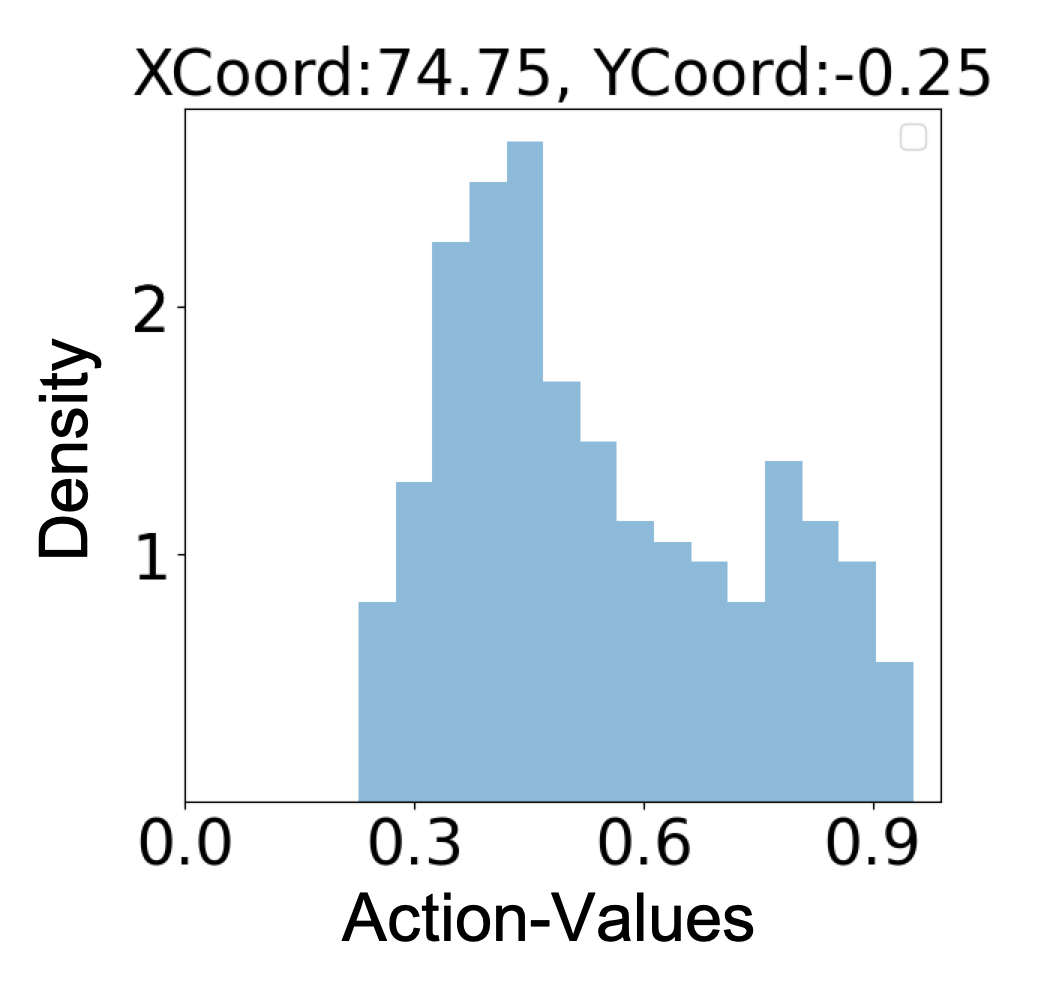
\includegraphics[scale=0.13]{figures/distribution_idx_21_XCoord_74.75_YCoord_-0.25-marked.png}
    % \end{minipage}\hfill
    % \begin{minipage}{0.12\textwidth}
    % 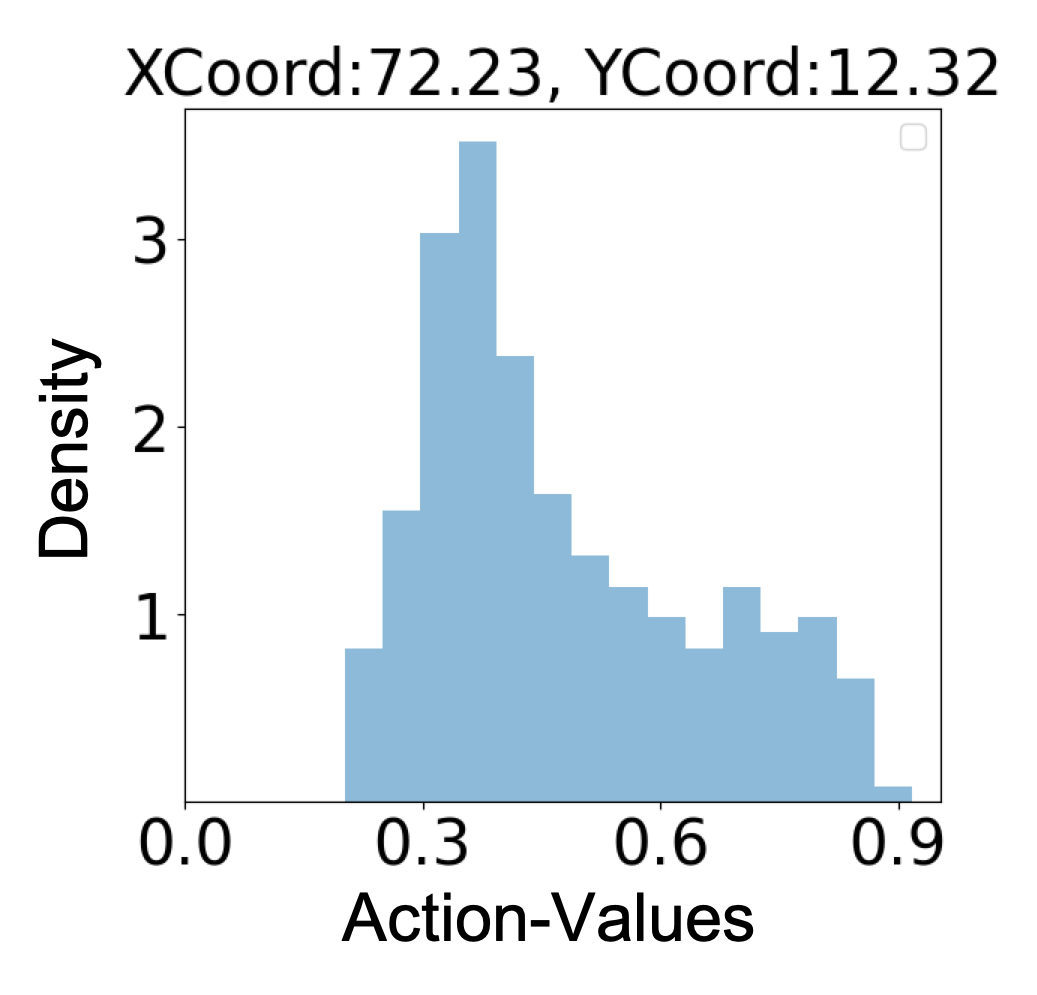
\includegraphics[scale=0.13]{figures/distribution_idx_22_XCoord_72.23_YCoord_12.32-marked.png}
    % \end{minipage}\hfill
    % \begin{minipage}{0.12\textwidth}
    % 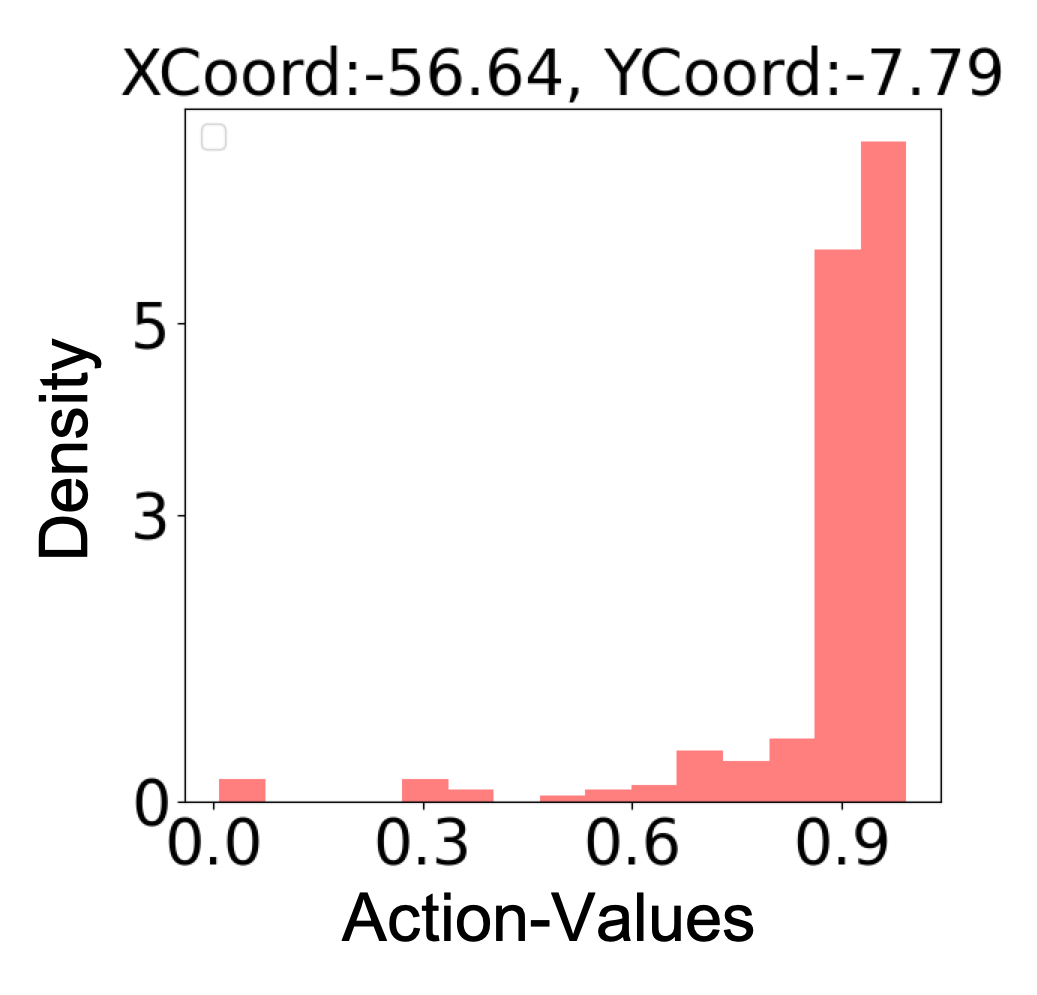
\includegraphics[scale=0.13]{figures/distribution_idx_35_XCoord_-56.64_YCoord_-7.79-marked.png}
    % \end{minipage}
    % \vspace{-0.1in}
    % \begin{minipage}{0.5\textwidth}
    % \centering
    % 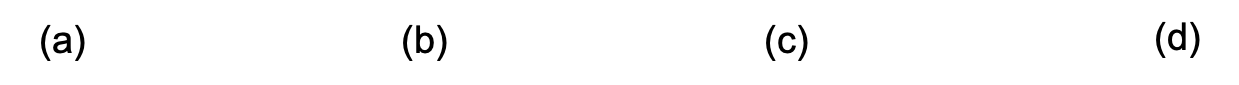
\includegraphics[scale=0.35]{figures/ice-hockey-view-label.png}
    % \end{minipage}
    % \vspace{-0.1in}
    % \begin{minipage}{0.4\textwidth}
    % 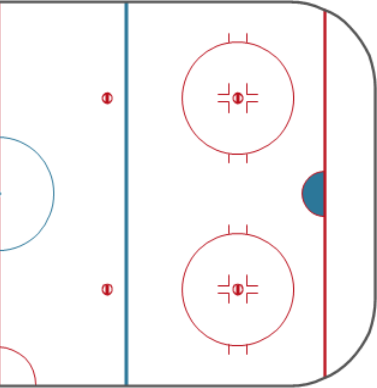
\includegraphics[scale=0.23]{figures/hockey-field-half.png}
    % \end{minipage}\hfill
    % \begin{minipage}{0.6\textwidth}
    %     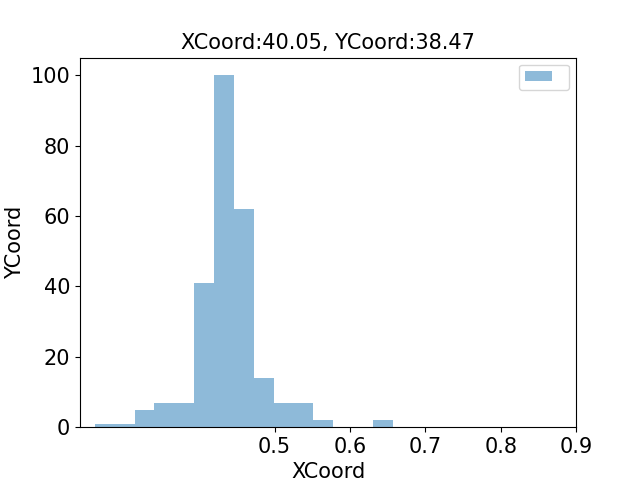
\includegraphics[scale=0.1]{figures/distrib_example_1_oct28.png}
    %     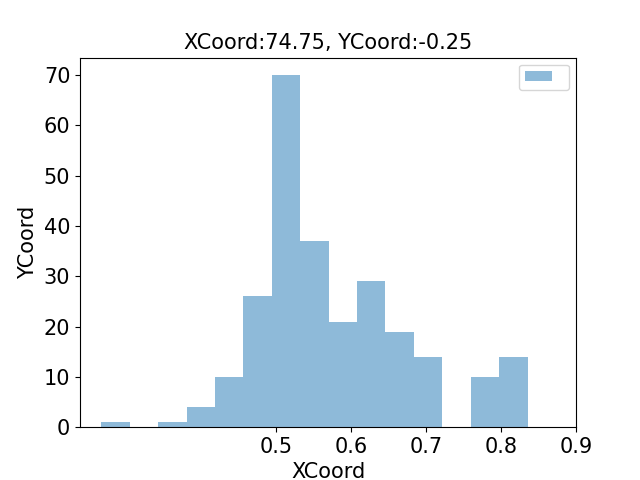
\includegraphics[scale=0.1]{figures/distrib_example_2_oct28.png}\\
    %     \includegraphics[scale=0.1]{figures/distrib_example_3_oct28.png}
    %     \includegraphics[scale=0.1]{figures/distrib_example_4_oct28.png}
    % \end{minipage}
    \vspace{-0.25in}
    \caption{The ice hockey rink, where players shoot the puck to their opponent's goal (on the right) in a match between Blues and Coyotes, 2018-19 NHL season. For quantifying the aleatoric uncertainty, we predict the distributions of future goals for the shots in positions (a) - (d), but the prediction (d) should be filtered since it is OoD (shooting from the deep backcourt is rare) and thus is likely to be incorrect (the predicted scoring chances are too large).}
    \label{fig:examples-distribution-ice-hockey}
    \vspace{-0.15in}
\end{figure}

In this paper, we design a data-driven RL framework for player evaluation. As Figure~\ref{fig:examples-distribution-ice-hockey} shows, instead of using a  conservative policy, we perform a post-hoc calibration of the learned action values by modeling two types of uncertainty:

% \begin{itemize}[leftmargin=*]
%   \item 
1) {\it Aleatoric uncertainty} captures the intrinsic stochasticity in game dynamics caused by stochastic rewards, transition dynamics, and policies. We show that this stochasticity can be captured by a distributional Bellman operator and propagated between action-value distributions by implementing Temporal-Difference (TD) learning with distributional RL.
  
2) {\it Epistemic uncertainty} is due to the finite training samples and OoD state-action pairs during testing. Online RL algorithms can overcome this uncertainty given sufficient exploration in the environment~\cite{Mavrin2019DistributionalRL}. However, when we have only a demonstration dataset with limited samples, the influence of epistemic uncertainty cannot be ignored, and thus we model it with feature-space densities from a Conditional Masked Auto-regressive Flow (CMAF).
% \end{itemize} 

Based on the uncertainty estimations, we develop a Risk-sensitive Game Impact Metric (RiGIM) for player evaluation. RiGIM filters the predictions for OoD samples and computes the impact of players' actions at each confidence level.
% by following the Value-at-Risk (VaR) method~\cite{duffie1997overview}
Empirical evaluation shows that RiGIM is highly correlated with ice hockey success measures when compared to other baselines. 
We measure the accuracy of action-value predictions and study the risk-sensitivity of \system by its correlations to the success measures at different confidence levels.

\paragraph{Contributions.} 1) we design a data-driven RL framework that enables post-hoc calibrations on action values according to their uncertainties. 2) we demonstrate how the distributional RL method and the CMAF model capture the aleatoric and epistemic uncertainties with action-value distributions and feature-space densities. 3) To the best of our knowledge, RiGIM is the first risk-sensitive metric for player evaluation.

\vspace{-0.05in}
\section{Related Works}
In this section, we introduce the previous works that are most related to our approach.
\paragraph{Uncertainty Estimation for RL.} 
An effective RL approach to guiding exploration and stabilizing policy is to utilize the uncertainties of future returns. To estimate the uncertainties, previous methods used the uncertainty Bellman equation~\cite{ODonoghue2018UncertaintyBellman}, bootstrap ensembles~\cite{Chen2017QEnsembles,Kumar2019Stable,Yu2020MOPO}, distributional value functions~\cite{Tang2018DistribExplore,Zhang2019QUOTA,Mavrin2019DistributionalRL}. Instead of separately capturing the epistemic and aleatoric uncertainties, these methods often quantify the overall uncertainty with a variance or entropy measure. 

\paragraph{Action Evaluation for Player.} 
The most common approach to player evaluation is to quantify the impact of their actions on game results~\cite{schwartz2017handbook}. Under this framework, \cite{Decroos2019Actions} trained a classifier to predict whether an action will be followed by a goal within a fixed look-ahead horizon.  
Some recent works also trained an action-value Q-function by dynamic programming~\cite{Routley2015Markov}, deep Sarsa~\cite{Liu2018DRL,Liu2020soccer} and Inverse RL~\cite{Luo2020IRL}. These methods compute an expected action-value without modeling their potential risk, and they commonly assume the training and testing datasets are identically distributed. 

% For the {\it online} RL problems where the agent can interact with the environment for collecting samples, the epistemic will shrink to zero when the agent learns the complete knowledge in the environment by running the exploration algorithm~\cite{Mavrin2019DistributionalRL,bellemare2017distributional}. In this case, the predictive uncertainty can directly captures the aleotoric uncertainty. However, for an {\it data-driven offline} RL problem (Section~\ref{subsec:offline-problem}), the training dataset is fixed and no exploration is allowed. The epistemic uncertainty cannot be eliminated since the environment commonly contains unexplored states and action by the demonstrate policy (with which $\dataset$ is collected). To develop an accurate value function for player evaluation, We must build separate model for capturing epistemic and aleotoric uncertainty.
% Unlike previous work that estimate uncertainty with complex approximation methods (e.g., variational model, ensemble models and Bayesian neural networks \textcolor{blue}{maybe add citation here}), in this work, we build deterministic model for capture uncertainty.

\section{An RL framework for Player Evaluation}
We represent the dynamics in ice hockey games with a Markov Game model and  introduce the motivation of estimating the aleatoric uncertainty and the epistemic uncertainty.

\subsection{Finite-Horizon Markov Game Model}
Player evaluation metrics commonly evaluate players by how much their actions influence the opportunity of scoring the next goal~\cite{Liu2018DRL,Decroos2019Actions,Sun2020Cracking}. Following this setting,  we divide an ice hockey game into goal-scoring episodes, so that each episode 1) begins immediately after a goal (or at the beginning of the game), and 2) terminates when the next goal is scored (or the end of the game is reached).

For a scoring episode of length $\horizon$, we model its dynamics with a finite-horizon Markov game model~\cite{Littman1994MarkovGame}$: G=(\mathcal{\MakeUppercase{\state}}, \boldsymbol{\mathcal{\MakeUppercase{\action}}}, P_{\mathcal{\MakeUppercase{\transition}}}, \boldsymbol{\MakeUppercase{\reward}}, \mathcal{\MakeUppercase{\observation}},\horizon,\gamma)$. 
% For the $\gameIndex^{th}$ episode in the training dataset $\dataset$, 
At a time step $t\in[0,\horizon]$, an agent $\agentIndex$ performs an action $\action_{\agentIndex,t} \in \mathcal{\MakeUppercase{\action}}_{\agentIndex}$ at a game state $\state_{t} \in \mathcal{\MakeUppercase{\state}}$ after receiving an observation $\observation_{t} \in \mathcal{\MakeUppercase{\observation}}$. 
This process generates the next state $\state_{t+1} \sim P_{\mathcal{\MakeUppercase{\transition}}}(\cdot|\state_t, \action_t)$ and a reward
$\reward_{k,t}=\MakeUppercase{\reward}_{\agentIndex}(\state_{t},\action_{\agentIndex,t})$. $\gamma$ is a discount factor.
In this paper, we consider two agents $\agentIndex\in\{Home, Away\}$ representing the home and away teams. The observed data $\dataset=[(\observation_1,\action_{\agentIndex,1},\boldsymbol{\reward}_{1}),(\observation_2,\action_{\agentIndex,2},\boldsymbol{\reward}_{2}),$ $\ldots,(\observation_t,\action_{\agentIndex,t},\boldsymbol{\reward}_{t}),\ldots]$ contains only the action $\action_{\agentIndex,t}$ performed by the team $\agentIndex$ who possesses the puck.  To alleviate partial observability, a game state includes the game history: $\state_{t} := (\observation_t,\action_{t-1},\observation_{t-1},\ldots,\observation_{0})$. The reward $\boldsymbol{\reward}_{t}$ is a 1-of-3 indicator vector that specifies which team ($Home, Away, Neither$) scores. We assign zeros to $\boldsymbol{\reward}_{t}$ until a team scores at the end of an episode.


% \subsection{Player Evaluation as an Offline RL Problem}
\subsection{Learning Action-Values from Offline Data}
\label{subsec:offline-problem}

As a data-driven behavior analytic tool, the player evaluation model assigns values to players' actions by learning from an offline dataset. Under this setting, previous works commonly~\cite{Routley2015Markov,Liu2018DRL,Liu2020soccer,Decroos2019Actions} utilized the same datasets for training and testing or assumed that the datasets are sampled from the same underlying distribution. However, in practice, since the behaviors of players may change when some team members (especially core players or the coach) are traded or hired during a season, there is no guarantee that the visitation frequency of state-action pairs is consistent in different games. It is natural to assume a distributional shift between the games in the training and testing dataset: while the value function is trained under one distribution, it will be evaluated on a different distribution.

% We define the player evaluation task as an offline Reinforcement Learning (RL) problem~\cite{Levine2020OfflineRL}. Unlike classic RL agent that are trained and tested under the given environments, the offline RL agent learns from a fixed dataset $\dataset$ without interacting with the environment or collecting additional transitions using the behavior policy. This setting is consistent with the ice hockey application, where RL is applied as a data-driven analytics tool for
% professional players instead of controlling artificial agents. Under this setting, the agent must learn action-value functions with the dataset of training games and evaluate performance of the players in testing games. The fundamental challenge of Offline RL is distributional shift: while value function trained under one distribution, it
% will be evaluated on a different distribution, due to the change in both visited states and demonstration policies (implemented by different teams). To derive a promising player evaluation, the agent must be aware the uncertainty of predictions (especially for the Out-of Distribution (OoD) states).

\paragraph{Calibration with Uncertainty.}
To alleviate the influence of distribution shift, offline RL algorithms~\cite{Levine2020OfflineRL} commonly discourage the visit to OoD state-action pairs by artificially lowering their values or adding penalties to their rewards. However, to evaluate players' performance, RL is employed as a policy evaluation tool instead of controlling players. The trajectories in testing games correspond to observed players' actions that cannot be changed or influenced by penalties. Instead, we perform a post-hoc calibration of the predicted action values by modeling their {\it epistemic uncertainty}, which is due to a lack of knowledge about OoD samples, and thus the resulting model is uncertain about the returns (Section~\ref{subsec:epistemic-uncertainty}). Since our goal is to develop a risk-sensitive player evaluation metric, we estimate distributions of action values to model their {\it aleatoric uncertainty}, which is due to the intrinsic stochasticity in the game dynamics (Section~\ref{subsec:aleatoric-uncertainty}).
In practice, the quantification of aleatoric uncertainty can be influenced by the input density (or the difference between training and testing distributions), so we filter the OoD samples with large epistemic uncertainty (Section~\ref{subsec:evaluation-metric}).

% The uncertainty of actions for a testing sample $(\Tilde{\state},\Tilde{\action})$ can be factorized into both the {\it epistemic} and the {\it aleatoric} uncertainty,
% % ~\cite{Smith2018Uncertainty,Hullermeier2021uncertainty,Mukhoti2021Uncertainty}, 
% where
% % \begin{enumerate}[nosep]
% \setlist[itemize]{leftmargin=*}
% \begin{itemize}
% \setlength\itemsep{0em}
%     \item Aleatoric uncertainty is due to the intrinsic stochasticity in the dynamics of ice hockey games. Since the transition and reward functions of ice hockey games are stochastic, the expected goals carry uncertainty.
%     \item Epistemic uncertainty is due to the model's lack of knowledge about the data $(\Tilde{\state},\Tilde{\action})$ (i.e., $(\Tilde{\state},\Tilde{\action})$ is Out-of-Distributed), and thus, the model is uncertain about the returns.
% \end{itemize}
% As a result, apart from the epistemic uncertainty due to distribution shift, the aleatory uncertainty (due to stochastic game dynamic) must be captured in order to develop a robust evaluation metric. In this work

% In the rest of this paper, we introduce the approach to capture aleatoric and epistemic uncertainty (Section~\ref{Sec:action-value-function}) and to estimate a risk-sensitive player evaluation metric (Section~\ref{Sec:evaluation-metric}).


% \subsection{Distributional Reinforcement Learning}
% \subsection{Distributional RL for Player Evaluation}
% Our approach of deriving a uncertainty-aware player evaluation metric is shown in Figure~xxx. We utilize distributional RL to learn an action-value function $Z(\state,\action)$ that predicts the distribution of expected future goals when a player perform an action $\action$ under a state $\state$. This distribution capture both the (partial\footnote{The distribution RL model might not capture the full epistemic uncertainty due to features collapse~\cite{Amersfoort2020Uncertainty}.}) {\it epistemic uncertainty} (induced by the OoD inputs $\state$ or $\action$ ) and the {\it aleatoric uncertainty} (induced by the stochasticity in environment dynamics)~\cite{Hullermeier2021uncertainty} of the player movement. We argue when measuring the risk of a player movement, only the aleotoric uncertainty should be counted (see Section~xxx). Based on samples from the predicted distribution, we compute a Vaule-at-Risk (VaR) Goal Impact metric  to value each player, based on the aggregated impact of their actions.

\section{Modelling the Uncertainty of Action Values }\label{Sec:action-value-function}

In this section, we introduce our method of modeling the aleatoric and epistemic uncertainty with a distributional-RL model and a feature-space density estimator (Figure~\ref{fig:model-architecture}).
% . Previous works demonstrate discriminate model and density 
% introduce how the our distributional-RL model and feature-space density estimator capture the aleatoric and epistemic uncertainty.

\begin{figure}[htbp]
    % \centering
    \vspace{-0.1in}
    \hspace{-0.1in}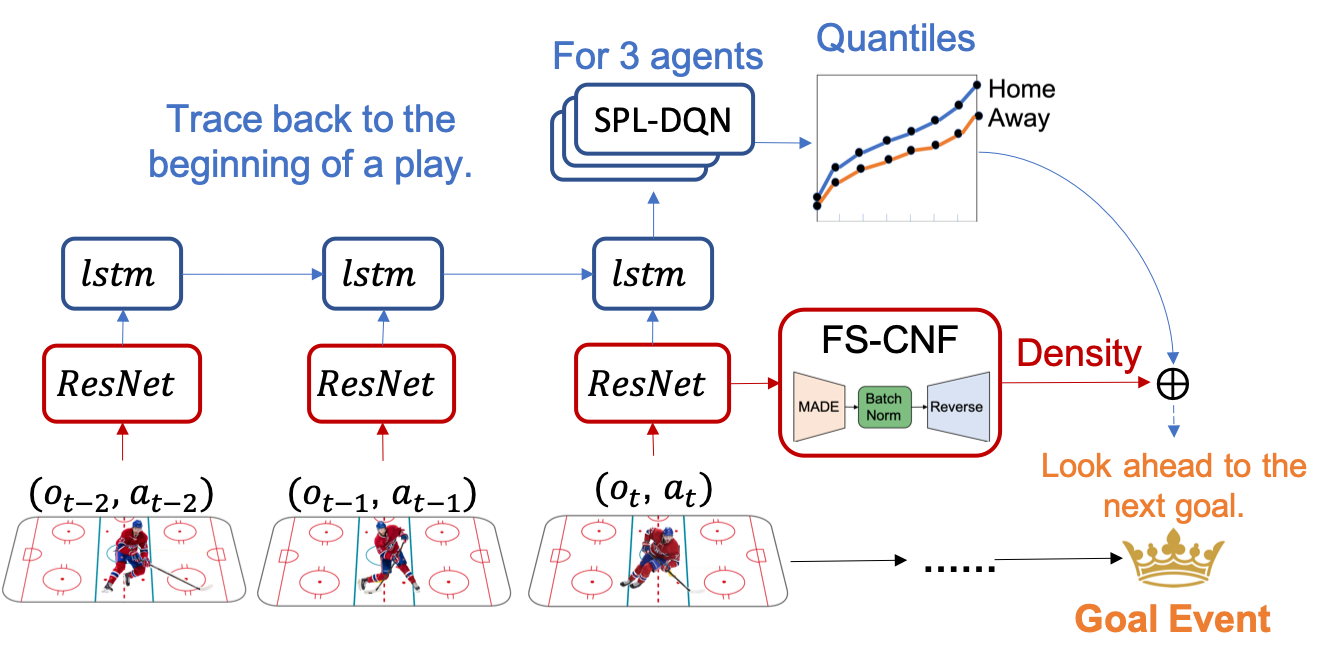
\includegraphics[scale=0.4]{figures/ice-hockey-net.png}
    \vspace{-0.3in}
    \caption{The architecture of our model: a play is a turn where one team attacks and the other defends. We stack residual networks with LSTM layers.
    % A play ends when a team loss the puck.
    }
    \label{fig:model-architecture}
    \vspace{-0.2in}
\end{figure}

% \subsection{Distribution Function for Action Values}
\subsection{Distributional RL for Aleatoric Uncertainty}\label{subsec:aleatoric-uncertainty}
Distributional RL learns the distribution of the random variable $Z_{\agentIndex}(\state_{t},\action_{t})$ that 
% \in P(\mathbb{R})^{\mathcal{\MakeUppercase{\action}}\times\mathcal{\MakeUppercase{\state}}}$ 
corresponds to the number of future goals when a player of team $k$ performs action $\action_{t}$ in state $\state_{t}$.  In other words, we can think of $Z_{\agentIndex}(\state_{t},\action_{t})$ as a random variable with outcomes corresponding to the sum of discounted rewards $\sum_{\iota=t}^{\horizon}\gamma^{\iota}\MakeUppercase{R}_{\agentIndex,\iota}(\MakeUppercase{\state}_\iota,\MakeUppercase{\action}_\iota)$, where $\MakeUppercase{\state}_t=\state_{t}$, $\MakeUppercase{\action}_t=\action_{t}$,
% $\reward_{\agentIndex,t}= \MakeUppercase{\reward}_{\agentIndex}(\state_{t},\action_{t})$, 
$\MakeUppercase{\state}_{\iota+1}$ is distributed according to $P_{\mathcal{\MakeUppercase{\transition}}}(\cdot|\MakeUppercase{\state}_\iota,\MakeUppercase{\action}_\iota)$ and $\MakeUppercase{\action}_\iota$ is distributed according to $\pi(\cdot|\MakeUppercase{\state}_\iota)$. 
% We use $T_{g}$ to denote the time step when the current goal-scoring episodes ends.
Following the Quantile-Regression (QR)-DQN method~\cite{bellemare2017distributional}, we represent the distribution of $Z$ by a uniform mixture of $N$ supporting quantiles:
\vspace{-0.15in}
\begin{equation}
    \hat{Z}_{\agentIndex}(\state_{t},\action_{t}) = \frac{1}{N}\sum_{\quantielIndex=1}^N \delta_{\theta_{\agentIndex,\quantielIndex}(\state_{t},\action_{t})}
    \vspace{-0.05in}
\end{equation}
where $\theta_{\agentIndex,\quantielIndex}$ estimates the quantile corresponding to the quantile level (or quantile index) $\hat{\tau}_i=\frac{\tau_{\quantielIndex-1}+\tau_\quantielIndex}{2}$ ($1\leq \quantielIndex\leq N$, and $\tau_\quantielIndex=\quantielIndex/N$) and  $\delta_{\theta_{\agentIndex,i}}$ denotes a Dirac distribution at $\theta_{\agentIndex,\quantielIndex}$. [$\theta_{\agentIndex,1},\dots,\theta_{\agentIndex,N}$] are monotonically increasing quantile values computed by the Non-Decreasing Quantile Function Network (NDQFN) by following~\cite{Zhou2021Quantile}. Since $\hat{Z}_{\agentIndex}$ is defined in a scoring episode, the support of predicted action-value distributions is in $[0,1]$.


% \end{enumerate}
% We provide a uncertainty model for ice hockey games as follows:
% \vspace{-0.15in}
% \begin{align}
%     ~\label{eqn:uncertainty}\\
%      H(Z|\Tilde{\state},\Tilde{\action},\dataset) = I(Z;\modelParamter|\Tilde{\state},\Tilde{\action},\dataset) + \expect_{ p(\modelParamter|\dataset)}(H(Z|\modelParamter,\Tilde{\state},\Tilde{\action}))\nonumber
% \end{align}
% where the mutual entropy  $I(Z;\modelParamter|\Tilde{\state},\Tilde{\action},\dataset)$ measures the amount of information we would gain about the model parameters $\modelParamter$ if we were to observe a new point data $\Tilde{\state},\Tilde{\action}$. When the information gain is large, $\Tilde{\state},\Tilde{\action}$ is OoD and our model has a poor knowledge about this situation. $\expect_{p(\modelParamter|\dataset)}(H(Z|\modelParamter,\Tilde{\state},\Tilde{\action}))$ acts as a Bayesian model for predictions. $p(\modelParamter|\dataset)$ forms an approximation to the distribution of sports dynamics and thus capture their intrinsic stochasticity.

% \subsection{Uncertainty Modelling with Value Function}
\paragraph{Distributional Bellman Operator.}
When a player in team $\agentIndex$ performs an action $\action_t$
% \sim\pi(\MakeUppercase{\action}_{t}|\MakeUppercase{\state}_{t}=\state_{t})$ 
at a state $\state_t$, the agent receives a reward $\MakeUppercase{\reward}_{\agentIndex}(\state_t,\action_t)$ and moves to a future state $\state_{t+1}\sim P_{\mathcal{\MakeUppercase{\transition}}}(\MakeUppercase{\state}_{t+1}|\state_t,\action_t)$ where the agent's next action $\action_{t+1}\sim\pi(\MakeUppercase{\action}_{t+1}|\MakeUppercase{\state}_{t+1})$. This stochastic process can be captured by a distributional Bellman operator $\mathcal{T}^{\pi}$~\cite{bellemare2017distributional}:
\vspace{-0.05in}
\begin{equation}
    \mathcal{T}^{\pi}{Z}_{\agentIndex}(\state_t,\action_t) \overset{\Delta}{:=} \MakeUppercase{\reward}_{\agentIndex}(\state_t,\action_t) + \gamma {Z}_{\agentIndex}(\MakeUppercase{\state}_{t+1},\MakeUppercase{\action}_{t+1})~\label{eqn:bellman-operator}
    \vspace{-0.05in}
\end{equation}
% where $\MakeUppercase{\state}^{\prime}$ and $\MakeUppercase{\action}$ are distributed according to $P(\cdot|\state,\action)$ and $ \pi_{\agentIndex}(\cdot|\MakeUppercase{\state}^{\prime})$. 
where $X\overset{\Delta}{:=}Y$ indicates that random variables $X$ and $Y$ follow the same distribution.
% Unlike $Q$-learning that estimate the expect value $\expect[Z^{\pi}(\state,\action)]$, distributional RL directly models the full distribution of $Z^{\pi}_{\agentIndex}$ to captures the uncertainty.
Based on the distributional Bellman operator, we estimate the supporting quantiles of $Z$ by minimizing the quantile Huber loss (with threshold $\eta$):
\vspace{-0.05in}
\begin{align}
    \frac{1}{N}\sum_{\quantielIndex=1}^N\sum_{\quantielIndex^{\prime}=1}^N\rho^{\eta}_{\hat{\tau}_\quantielIndex}(\reward+\gamma\theta_{\quantielIndex^{\prime},\agentIndex}(\state_{t+1},\action_{t+1})-\theta_{\quantielIndex,\agentIndex}(\state_{t},\action_{t})) \text{ where }\nonumber~\label{eq:huber}
\end{align}
\vspace{-0.2in}
\begin{align}
    \begin{split}
    \rho_{\tau}^{\eta}(\sigma) = |\tau - \mathbb{I}_{\sigma<0}|\mathcal{L}_{\eta}(\sigma),~\mathrm{with} \\
    \mathcal{L}_{\eta}(\sigma) = \begin{cases}
    \tfrac12 \sigma^2, & |\sigma| \leq \eta\\
    \eta(|\sigma|-\frac12 \eta), & \mathrm{otherwise}.
\end{cases}
\end{split}
\vspace{-0.05in}
\end{align}

{\it Illustration of Temporal Projection}. Figure~\ref{fig:temporal-plot} illustrates the mean $\pm$ standard deviation of the action-values sampled from the predicted distributions $\hat{Z}(\state,\action)$, where $\state$ and $\action$ follow the players' movements in a match between the Flyers (Home team) and the Maple Leafs (Away team) on March 15, 2019. The figure plots values
of the three output nodes. We highlight critical events and
match contexts to show the context-sensitivity of our predictions. 
\vspace{-0.15in}
\begin{figure}[htbp]
    \centering
    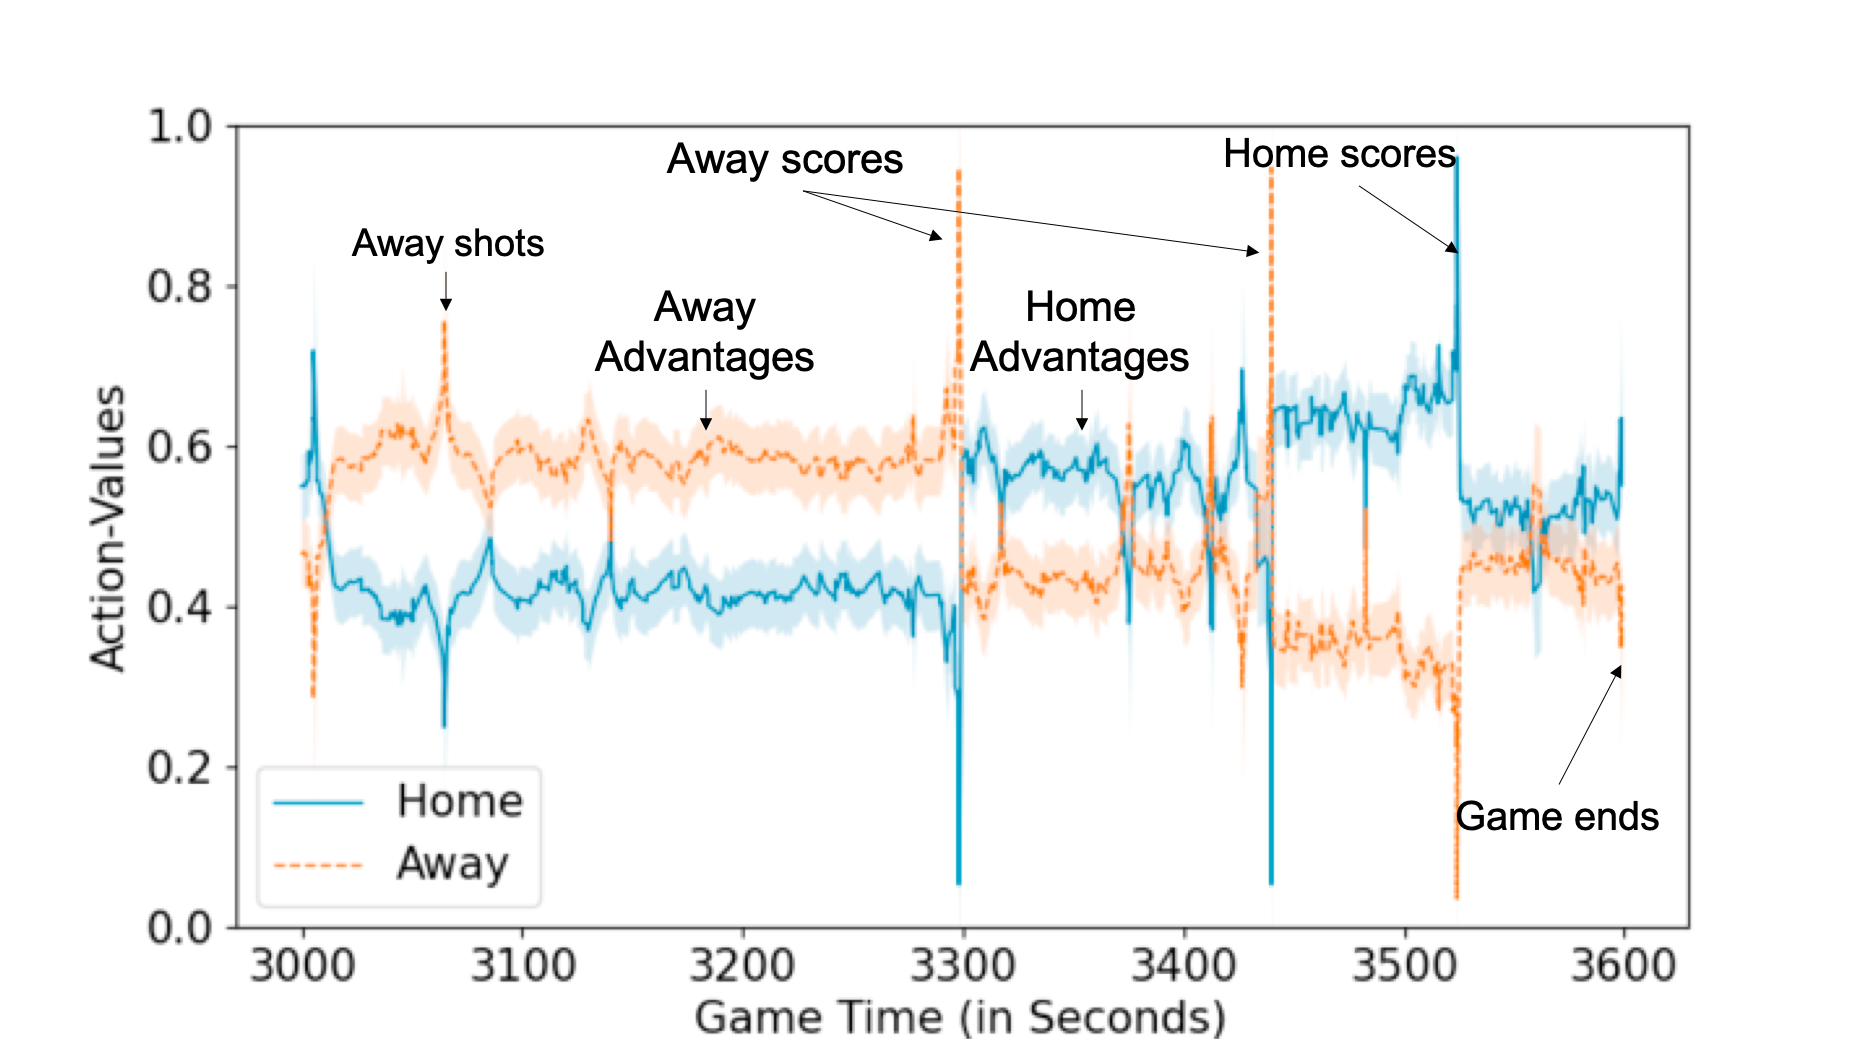
\includegraphics[scale=0.27]{figures/temporal-visualization-marked.png}
    \vspace{-0.25in}
    \caption{Temporal projections of the samples (mean $\pm$ standard deviation) from the predicted distributions at each time step.}
    \label{fig:temporal-plot}
    \vspace{-0.1in}
\end{figure}

We show that the predicted distribution of action values can measure the aleatoric uncertainty.

\begin{proposition}
Assume Bellman consistency  $\hat{\boldsymbol{Z}} \overset{\Delta}{:=} \MakeUppercase{\boldsymbol{\reward}} + \gamma \boldsymbol{P}^{\pi}\hat{\boldsymbol{Z}}$ 
where $\hat{\boldsymbol{Z}}$, $\boldsymbol{\MakeUppercase{\reward}}$ are vector-valued random variables and $\boldsymbol{P}^{\pi}$ is the transition matrix of the stationary policy $\pi$, so $P^{\pi}_{(\state,\action),(\state^{\prime},\action^{\prime})}=P(\state^{\prime}|\action,\state)\pi(\action^{\prime}|\state^{\prime})$. Then the uncertainty of action-value distributions $\hat{\boldsymbol{Z}}$ under an entropy measure $H(\cdot)$ is given by:
\begin{align}
    H(\hat{\boldsymbol{Z}}) = H[\boldsymbol{\MakeUppercase{\reward}}]-|\mathcal{\MakeUppercase{\action}}||\mathcal{\MakeUppercase{\state}}|\log(1-\gamma)+\log|\text{det}(\mathbf{d}^{\pi})|
\end{align}
where $\mathbf{d}^{\pi}=(1-\gamma)(I-\gamma \boldsymbol{P}^{\pi})^{-1}\in[0,1]^{|\MakeUppercase{\state}||\MakeUppercase{\action}|\times|\MakeUppercase{\state}||\MakeUppercase{\action}|}$ is the induced matrix for distributions over state-action tuples by following policy $\pi$ and transition $P_{\mathcal{\MakeUppercase{t}}}$. 
\end{proposition}

The proof is in Appendix B.1. Proposition 1 disentangles the entropy of $\boldsymbol{Z}$ into 1) the entropy of reward variables that quantifies the uncertainty of current rewards, 2) the uncertainty induced by the discount factor, which determines how much the current uncertainty estimation should be influenced by the stochasticity of future rewards or transitions (i.e., a small $\gamma$ reduces this influence), and 3) a log-absolute determinant of the induced distribution matrix, which measures the amount of stretch or change that the transition function $P_{\mathcal{\MakeUppercase{\transition}}}$ and the policy $\pi$ apply to the initial state-action distribution.
% factor by which the function expands or shrinks volumes near

Proposition 1 suggests that the key components for representing the aleatoric uncertainty can be captured by $Z$ when learning leads to Bellman consistency.  However, in practice,  the estimation of $Z$ cannot be well generalized to all samples because of insufficient exploration or limited training data, so we need to estimate their epistemic uncertainty. 


% \begin{proposition}
% Assume the Bellman consistency holds by $\hat{Z}(\state_t,\action_t) \overset{\Delta}{:=} \MakeUppercase{\reward}(\state_t,\action_t) + \gamma \hat{Z}(\MakeUppercase{\state}_{t+1},\action_{t+1})$ 
% where $\MakeUppercase{\state}_{t+1}$ follows $ P_{\mathcal{\MakeUppercase{\transition}}}(\cdot|\state_{t},\action_{t})$ and
% % and ${\action}_{t+1}\sim\pi(\cdot|\MakeUppercase{\state}_{t+1})$
% ${\action}_{t+1}=\argmax_{\action_{t+1}} \expect_{P_{\mathcal{\MakeUppercase{\transition}}},\MakeUppercase{\reward}}[\hat{Z}(\state_{t+1}, \action_{t+1})]$
% , let $\hat{Z}(\state_{t},\action_{t};\dataset)$ be the distribution function learned by the training dataset $\dataset$ and let $\gamma=1$, the uncertainty capture by the predicted distribution under an entropy measure $H(\cdot)$ in a MDP with a finite horizon $\horizon$ is given by:
% \begin{align}
%     & H[Z(\state_{t},\action_{t};\dataset)]=(\horizon-t)\cdot\sum_{\Tilde{\state},\Tilde{\action}}\hat{d}_{{\state}_{t},{\action}_{t}}^{\pi}(\Tilde{\state},\Tilde{\action};\dataset)H(\MakeUppercase{\state}^{\prime}|\Tilde{\state},\Tilde{\action})\nonumber
%     % & \text{and } \phi(\Tilde{\state},\Tilde{\action};\dataset)=H(\MakeUppercase{\state}^{\prime}|\Tilde{\state},\Tilde{\action};\dataset) + H(\MakeUppercase{\action}^{\prime}|\MakeUppercase{\state}^{\prime},\Tilde{\state},\Tilde{\action};\dataset)
% \end{align}
% where $H[Z(\cdot)]$ denotes the entropy of predicted distribution and $\hat{d}_{{\state}_{t},{\action}_{t}}^{\pi}(\Tilde{\state},\Tilde{\action};\dataset)$ denotes the probability of visiting state-action pair $(\Tilde{\state},\Tilde{\action})$ from $({\state}_{t},{\action}_{t})$ within $(\horizon-t)$ steps.
% \end{proposition}

% The proof is in Appendix~\textcolor{blue}{xx}. Note that we define a deterministic reward function (so $H(\MakeUppercase{\reward})=0$). 
% % and the entropy of reward variable given a state-action pair is zero. 
% A stochastic reward function adds complexity to proof since $H(\MakeUppercase{\reward}+Z(\cdot))\leq H(\MakeUppercase{\reward})+H(Z(\cdot))$. This upper bound could be loose \textcolor{blue}{(depending on the assumptions of their parametric distributions.)} and the equivalence holds only when $H(\MakeUppercase{\reward})=0$ or $H(Z(\cdot))=0$.

% Proposition 1 shows that the intrinsic stochasticity in the environment for a given sample $(\Tilde{\state},\Tilde{\action})$ (denoted as $H(\MakeUppercase{\state}^{\prime}|\Tilde{\state},\Tilde{\action})$) can be captured by the predicted distribution of $Z|_{\state_{t},\action_{t}}$. However, the estimation of visiting probability
% % , entropy terms are 
% is based on training data $\dataset$ while the true visiting probability $d^{*}_{\state_t,\action_t}(\cdot)$ 
% % and entropy $\phi^{*}(\cdot)$ 
% follows the testing policy. 
% For a testing sample $(\Tilde{\state},\Tilde{\action})$ with small a density on the training distribution, it is difficult to drive an accurate estimation of entropy due to the lack of exploration. 
% The aleatoric uncertainty could be influenced by the epistemic uncertainty of $(\Tilde{\state},\Tilde{\action})$.


% Distributional RL directly predicts the distribution of discounted future goal $Z$ whose range is $[0, 1]$. Given a new data point $\Tilde{\state},\Tilde{\action}$, we can calculate its (approximated) predictive uncertainty $H(Z|\Tilde{\state},\Tilde{\action},\dataset)$ ($H(\cdot)$ indicates entropy) with the samples [$\theta_{1},\dots,\theta_{N}$]~\footnote{The sampling method is Inverse Transform Sampling.} from $p(Z)$. 

\vspace{-0.05in}
\subsection{Density Estimator for Epistemic Uncertainty}\label{subsec:epistemic-uncertainty}
% \paragraph{Feature-Space Density Model.}
By definition, epistemic uncertainty is higher for the OoD samples. An effective approach to detect OoD samples is to estimate the density for each sample in the training data distribution
% (e.g., novelty detection)
~\cite{Mukhoti2021Uncertainty}, so that an OoD sample has low density while an InD sample has high density. To learn the training data distribution, we utilize a Conditional Masked Auto-regressive Flow (CMAF).
% \textcolor{blue}{shall we discuss why we need the density method?}

{\it CMAF}~\cite{Papamakarios2017MAF} estimates the density of input variables in the training data distribution with an auto-regressive constraint, and to make MAF more sensitive to the abnormal predictions in OoD samples, the density model is conditioned on the expected returns of action-value distributions, so $p(\boldsymbol{\datapoint}|{\condition})=\sum_{i}p(\datapoint_{i}|\datapoint_{1:i-1},{\condition})$  where ${\condition}:=\{\expect[Z_{\agentIndex}(\state,\action)]\}_{\agentIndex=1}^{\MakeUppercase{\agentIndex}}$ and $\boldsymbol{\datapoint}:=(\observation,\action)$ (we use $\observation$ instead of $\state$ since a large input dimension influences the accuracy of estimation). We implement $p(\datapoint_{i}|\datapoint_{1:i-1},\condition)=\mathcal{N}(\datapoint_{i}|\mu_{i},(\text{exp}(\alpha_{i}))^{2})$ where $\mu_{i}=\psi_{\mu_{i}}(\datapoint_{1:i-1},\condition)$ and $\alpha_{i} = \psi_{\alpha_{i}}(\datapoint_{1:i-1},\condition)$. The neural function $\psi$ is implemented by stacking multiple MADE layers~\cite{Dias2020NFAnomaly}.
% , where the autoregressive property is enforced by multiplying the weight matrices of MADE with binary masks.
% Previous works~\cite{Schmidt2019noveltyMAF,Dias2020NFAnomaly} demonstrated the novelty-detection performance of MAF in the time series data with spatial-temporal features.
% Based on the distance-aware features  $\feature=f(\state,\action;\modelParamter_{\mathcal{\MakeUppercase{\feature}}})$, we follow~\cite{Mukhoti2021Uncertainty} and estimate the input density $q(\feature)$ by 1) dividing the $\expect(Z(\state,\action))\in[0,1]$ into $\splitnum$ classes $\{\Tilde{z}_{1},\dots,\Tilde{z}_{\MakeUppercase{\splitnum}}\}$ and 2) building a Gaussian Discriminant Analysis (GDA) model, a GMM with a single Gaussian mixture component per class $q(\feature|\Tilde{z}_{\splitnum})$. We fit each class component of the GDA by computing the empirical mean and covariance, per slot, of the feature vectors $\feature$.
% % , which are the outputs of the last residual layer of the model computed on the training samples ($(\state,\action)\in\dataset$).  
% At test time, we compute the epistemic uncertainty by evaluating the marginal likelihood of the feature representation under our density by $q(\feature)=\sum_{\Tilde{z}_{m}} q(\feature|\Tilde{z}_{m}) q(\Tilde{z}_{m})$.

\vspace{-0.05in}
\section{Player Evaluation}\label{Sec:player-evaluation}

In this section, we introduce our player evaluation metric and show examples of risk-sensitive rankings.

\subsection{Risk-sensitive Impact Metric}\label{subsec:evaluation-metric}
\paragraph{Measuring Risk.} We measure the risk of a player's movement with the aleatoric uncertainty since modeling the intrinsic stochasticity of the game dynamics is consistent with the goal of sports analytics.
However, as Figure~\ref{fig:spatial-uncertainty} shows, when we quantify the aleatoric uncertainty with our distributional RL model, the performance can be influenced by the density of input samples. This influence can become more apparent with a distributional shift between training and testing data.
\vspace{-0.15in}
\begin{figure}[htbp]
    % \begin{minipage}[b]{0.48\textwidth}
    % \begin{minipage}{0.5\textwidth}
    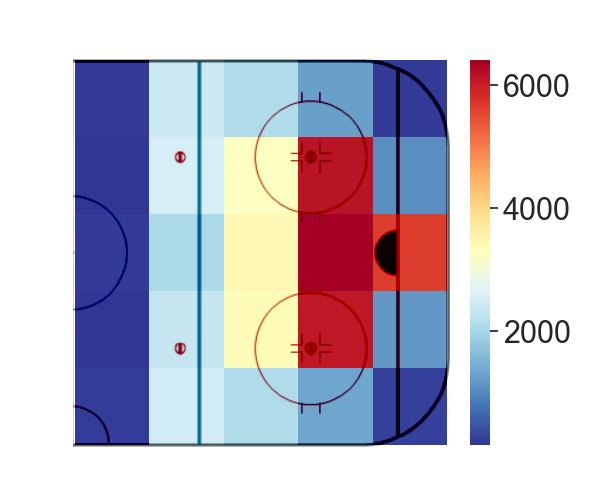
\includegraphics[scale=0.2]{figures/spatial_train_num_blend.png}
    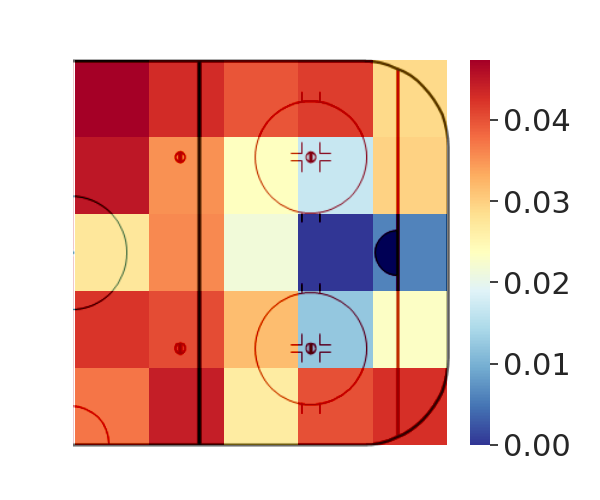
\includegraphics[scale=0.2]{figures/spatial_std_diff_blend.png}
    % \end{minipage}
    \vspace{-0.3in}
    \caption{We discretize the ice hockey rink into 5$\times$5 regions. For each region, the {\it left} heatmap shows the numbers of shots in the {\it training dataset}, and the {\it right} heatmap shows the Mean Absolute Error (MAE) between the estimated and the real aleatoric uncertainty for shot values in the {\it testing dataset}. We observe a negative correlation (-0.761) between the density and the MAE across these regions.}
    \label{fig:spatial-uncertainty}
    \vspace{-0.1in}
    % \end{minipage}
\end{figure}

An effective approach to verify whether $\hat{Z}_{\agentIndex}(\state,\action)$ accurately captures the true aleatoric uncertainty is to examine the scale of epistemic uncertainty for each input datum $(\state,\action)$~\cite{Mukhoti2021Uncertainty}: 1) a high input density ($p(\cdot|\condition)\geq\epsilon$) indicates low epistemic uncertainty,
(i.e., $(\state,\action)$ is InD)
and we can trust the aleatoric uncertainty estimated by distributional RL. 2) a low input density ($p(\cdot|\condition)<\epsilon$) indicates high epistemic uncertainty (i.e., the input is OoD, and we do not use the corresponding estimation). In practice, $\epsilon$ is determined based on the validation dataset.

\paragraph{Action Impact.}
The {\it impact} $\impact(\state,\action)$ measures how much an action $\action$ changes the future return of a player's team. In terms of the value function, this is the change in action value due to a player’s movement. 
% \textcolor{blue}{The impact can be visualized as the difference between successive points in the action-value ticker (Figure xxx).} 
Previous works~\cite{Routley2015Markov,Liu2018DRL,Decroos2019Actions} computed the impact with the expected next-goal return $Q(\state_{t},\action_{t})=\expect[Z(\state_{t},\action_{t})]$. $Q(\cdot)$ does not take into account the inherent variability of the returns and thus cannot estimate the risk of an action. As Figure~\ref{fig:distribution-of-shot-returns} shows, actions with the similar expected return can have significantly different risk-sensitive estimates. To understand how players respond to risk, we propose a Risk-sensitive Game Impact Metric (\system) based on $\hat{Z}_{\agentIndex}(\state,\action)$ and $p(\cdot|\condition)$:
% \vspace{-0.05in}
\begin{align}
    &\impact_{\agentIndex}(\state_{t+1},\action_{t+1},\confidence)=\big[\hat{Z}^{\confidence}_{\agentIndex}(\state_{t+1},\action_{t+1})-
    % 1/\gamma \expect_{\state_{t},\action_{t}}[
    \hat{Z}^{\confidence}_{\agentIndex}(\state_{t},\action_{t})\big]\mathbb{I}_{p(\cdot|\condition)\geq\epsilon}
    % ]
    \nonumber\\
    &\sys_{\playerId}(\confidence)=\sum_{(\state,\action)\in\dataset^{\prime}}n(\state,\action,\playerId)\times\impact_{\agentIndex}(\state,\action,\confidence)\label{eqn:RIGIM}
    \vspace{-0.1in}
\end{align}
where $\confidence\in[0,1]$ is the confidence level, $Z^{\confidence}$ denotes the $(1-\confidence)^{th}$ quantile in $Z(\cdot)$ and $n(\state,\action,\playerId)$ denotes the number of times that a player $\playerId$ performs action $\action$ at a state $\state$ in the testing dataset $\dataset^{\prime}$. We omit the term $\reward_t$ since $\reward_{t}=0$ except at scoring step $T$, and $\state_{T}$ is the terminal state of a scoring episode.
% (i.e., $\state_{T+1}$ does not exist). 
% In the expectation term, only the data points $\state_{t},\action_{t}$ whose next state is $\state_{t+1}$ will be measured. 
$\impact(\cdot)$ can either be 1) risk-averse (with a large $\confidence$), with better sensitivity to bad outcomes or 2) Risk-seeking (with a small $\confidence$), with better sensitivity to positive outcomes.
\vspace{-0.15in}
\begin{figure}[htbp]
    % \begin{minipage}[b]{0.48\textwidth}
    % \begin{minipage}{0.5\textwidth}
    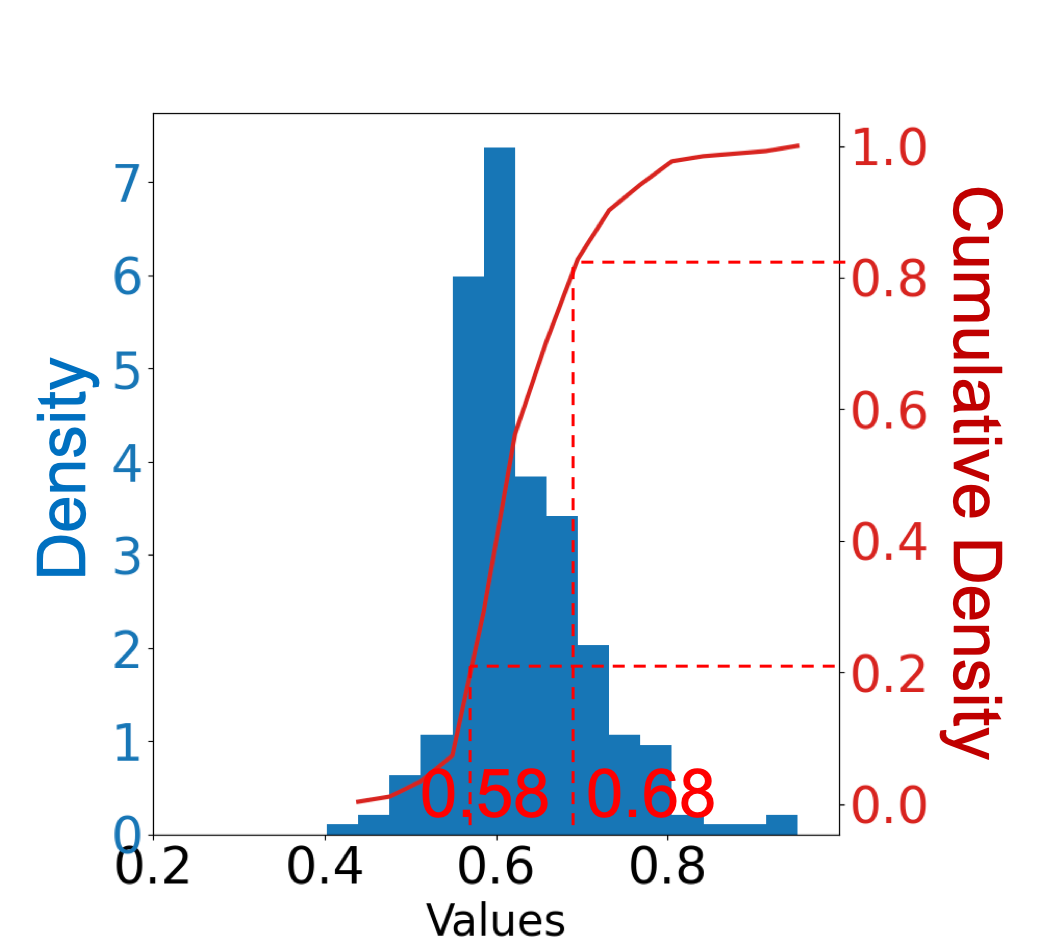
\includegraphics[scale=0.15]{figures/density_idx_7_XCoord_85.69_YCoord_-21.88_marked.png}
    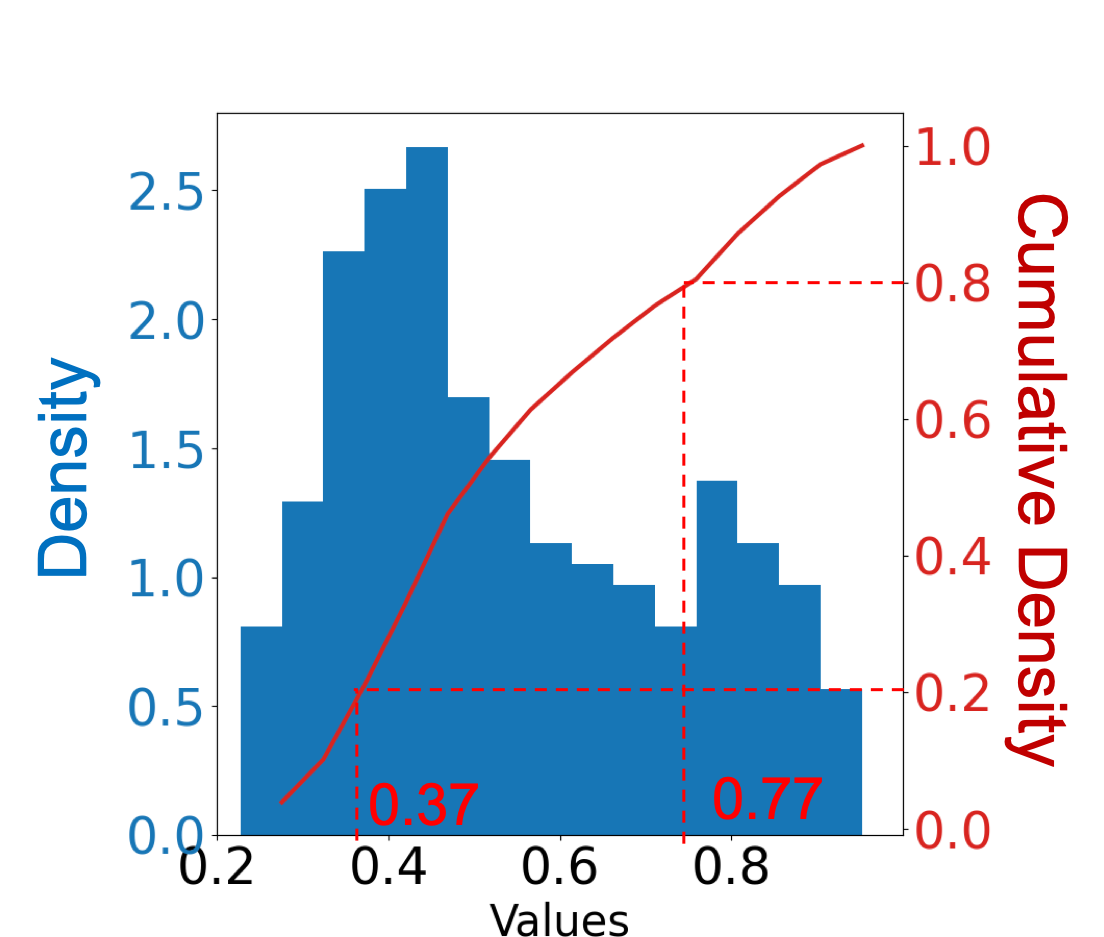
\includegraphics[scale=0.15]{figures/density_idx_21_XCoord_74.75_YCoord_-0.25_marked.png}
    \vspace{-0.1in}
    % \end{minipage}
    \caption{The next-goal distributions of two shots under different contexts. Both distributions have a similar expectation (around 0.6), but the first shot is less risky than the latter shot since the first shot has 1) a larger risk-averse estimate (when $c=0.8$, $0.58 > 0.37$) and 2) a smaller risk-seeking estimate (when $c=0.2$, $0.68 < 0.77$). }
    \label{fig:distribution-of-shot-returns}
    \vspace{-0.15in}
    % \end{minipage}
\end{figure}

\subsection{Case Study: Player Ranking in Testing Games}
We rank players according to their \system scores in testing games (check the experiment setting in Section~\ref{Sec:experiment}) at different confidence levels. Table~\ref{table:player-ranking-0.2} shows a {\it risk-seeking} ranking (with confidence $\confidence=0.2$),  which favors offensive players (e.g., Centres (C)) with strong scoring ability. Aleksander Barkov, who scores most points in the testing games, is captured by this ranking. When we set confidence $\confidence$ to 0.8, Table~\ref{table:player-ranking-0.8} shows a {\it risk-averse} ranking which highlights players in defensive positions (e.g., Defensive (D)). John Klingberg, the defenseman with the most assists, is listed as a top-10 player. 
% We find the risk-seeking players generally score more goals that the risk-averse player, which is consitant with 

% according to their performance in the testing games. 
\begin{table}[htbp]
\centering
\resizebox{0.45\textwidth}{!}{
\begin{tabular}{ccccccc}
\toprule
Player Name  & Position & Team  & P & A & G & \sys \\ \hline
Jonathan Toews & C & CHI & 10 & 5 & 5 & 14.72\\ 
Anze Kopitar & C & LAK & 12 & 9 & 3 & 14.55\\ 
Vincent Trocheck & C & FLA & 8 & 5 & 3 & 14.02\\ 
Tomas Hertl & C & SJS & 12 & 8 & 4 & 13.97\\ 
John Tavares & C & TOR & 12 & 3 & 9 & 13.92\\ 
Tyler Seguin & C & DAL & 18 & 12 & 6 & 13.71\\ 
Leon Draisaitl & C & EDM & 16 & 8 & 8 & 13.16\\ 
Aleksander Barkov & C & FLA & 19 & 14 & 5 & 12.63\\ 
Sean Couturier & C & PHI & 11 & 6 & 5 & 12.62\\ 
Nathan MacKinnon & C & COL & 12 & 6 & 6 & 12.48\\ 
\bottomrule
\end{tabular}
}
\vspace{-0.1in}
\caption{Top 10 players in testing games with confidence 0.2.}
\vspace{-0.05in}
\label{table:player-ranking-0.2}
\end{table}

\begin{table}[htbp]
\centering
\resizebox{0.45\textwidth}{!}{
\begin{tabular}{ccccccc}
\toprule
Player Name  & Position & Team  & P & A & G & \sys \\ \hline
Radek Faksa & C & DAL & 6 & 3 & 3 & 2.74\\ 
Leon Draisaitl & C & EDM & 16 & 8 & 8 & 2.51\\ 
John Klingberg & D & DAL & 10 & 9 & 1 & 2.46\\ 
Esa Lindell & D & DAL & 3 & 1 & 2 & 2.29\\ 
Connor McDavid & C & EDM & 18 & 11 & 7 & 2.23\\ 
Tomas Hertl & C & SJS & 12 & 8 & 4 & 1.93\\ 
Miro Heiskanen & D & DAL & 5 & 3 & 2 & 1.86\\ 
Elias Pettersson & C & VAN & 8 & 6 & 2 & 1.79\\ 
Tyler Seguin & C & DAL & 18 & 12 & 6 & 1.78\\ 
Roope Hintz & LW & DAL & 11 & 7 & 4 & 1.77\\ 
\bottomrule
\end{tabular}
}
\vspace{-0.1in}
\caption{Top 10 players in testing games with confidence 0.8.}
\vspace{-0.15in}
\label{table:player-ranking-0.8}
\end{table}

\section{Empirical Evaluation}\label{Sec:experiment}

\paragraph{Experiment Settings.} Our experiments utilize a \textbf{game events} dataset for the entire 2018-2019 National Hockey League (NHL) season, which contains 4,534,017 events, covering 31 teams, 1,196 games and 1,003 players. Each  dataset consists of events around the puck. Each event records the identity and action of the player possessing the puck, with time stamps and features of the game context (Appendix A.1. contains a complete list of game features). We divide the dataset into a training set (80\%), a validation set (10\%), and a testing set (10\%) according to game dates, so that games in the testing set happened after the games in the training and validation set. To predict the action values in the testing games, the metric must remain robust to OoD data points.
% \textcolor{blue}{is there a way to prove there are OoD datapoints, I guess some game statistics will help.} 
We implement 5 independent runs and report the results.

\paragraph{Comparison Metrics.} We employ an ablation design that iteratively removes parts from \system.  {\bf GIM} removes the uncertainty estimator by directly using a Deep Recurrent Q-Network for estimating action values~\cite{Liu2018DRL}. {\bf T0-GIM} removes the recurrent model and uses a Deep Q-Network (DQN) for the value function. We then replace the RL framework with a supervised learning framework for estimating action values by following {\bf VAEP}~\cite{Decroos2019Actions}. Instead of using function approximators, {\bf Scoring Impact (SI)}~\cite{Routley2015Markov} implements the tabular-based value iteration algorithm for computing action values from discretized spatial and temporal features. {\bf Expected-Goal(EG)} metric directly uses the expected action values instead of impact values for measuring player performance. The last 
% two
metric {\bf  Plus-Minus ($+/-$)}
% and {\bf Win Above Replacement (WAR)} are 
is based on game statistics and measures the value(goal)-gain with and without the player on ice. We summarize these metrics in Table~\ref{table:summary-baseline}.

\newcommand{\xmark}{\ding{55}}%
\newcommand{\cmark}{\ding{51}}
\begin{table}[htbp]
\resizebox{0.5\textwidth}{!}{
    \begin{tabular}{ccccccc}
    \toprule
    Method & \begin{tabular}[c]{@{}l@{}}Risk-\\ Aware\end{tabular} & \begin{tabular}[c]{@{}l@{}}History-\\ Aware\end{tabular} & \begin{tabular}[c]{@{}l@{}}RL-\\Based\end{tabular} & \begin{tabular}[c]{@{}l@{}}Continuous\\ Feature\end{tabular} &
    \begin{tabular}[c]{@{}l@{}}Impact-\\Based\end{tabular} &
    \begin{tabular}[c]{@{}l@{}}Context-\\ Aware\end{tabular} \\ \hline
    $+/-$ & \xmark  & \xmark  & \xmark   & \xmark   & \xmark  & \xmark  \\
    % WAR & \xmark  & \xmark  & \xmark   & \xmark   & \xmark  & \xmark  \\
    EG & \xmark  & \xmark  & \xmark   & \xmark   & \xmark  & \cmark \\
    SI & \xmark  & \xmark  & \xmark   & \xmark   & \cmark  & \cmark \\
    VAEP & \xmark  & \cmark  & \xmark   & \cmark  & \cmark  & \cmark \\
    T0-GIM & \xmark  & \xmark  & \cmark   & \cmark  & \cmark  & \cmark \\
    GIM & \xmark  & \cmark  & \cmark   & \cmark  & \cmark  & \cmark \\
    % Na-\system & \cmark  & \cmark  & \cmark   & \cmark  & \cmark  & \cmark \\ 
    \bottomrule
    \end{tabular}
}
\vspace{-0.1in}
\caption{A summary of the baseline metrics for player evaluation.}
\vspace{-0.2in}
~\label{table:summary-baseline}
\end{table}

To study how well our CMAF boosts model performance, we compare 1) a Gaussian Discriminant Analysis {\bf (GDA)-\system} metric that replaces CMAF with GDA by following~\cite{Mukhoti2021Uncertainty}, and 2) a Naive {\bf (Na)-\system} metric that removes the epistemic uncertainty estimator and uses only the distributional RL model to compute players' impact. Appendix A.2 and A.3 include our implementation details.

\subsection{Player Evaluation Performance: Correlations with Standard Success Measures}

We compute the correlations between player ranking metrics and success measures on the testing games in an NHL season. The standard success measures include Assist (A), Goal (G), Game Winning Goal (GWG), Overtime Goal
(OTG), Short-handed Goal (SHG), Power-play Goal (PPG),
Point (P), Short-handed Point (SHP), Power-play Point
(PPP),  Penalty Minute (PIM), Time On Ice (TOI), and Shots (S). These
are commonly used measures from the NHL official website \footnote{\url{http://www.nhl.com/stats/skaters}}.

Table~\ref{table:Correlations} shows the average correlations in 5 independent runs on the testing dataset (Check Table C.1 in Appendix for the mean $\pm$ standard deviation results.). Our \system metric achieves the highest correlations with 8 out of 12 success measures. If we remove CMAF or replace it with other uncertainty estimators, most correlations become weaker except the correlations with the SHP and SHG measures. SHP and SHG rarely happen in a game season (scoring with fewer players on ice is difficult); CMAF detects this phenomenon and assigns small densities to corresponding events. Some of these events can be filtered by CMAF, and thus our correlations with SHP and SHG are less significant. For the risk-neutral metrics, their performance is generally less satisfying when compared with risk-aware metrics, especially for the $+/-$ metric, which shows the importance of capturing risk and modeling the context features.

\begin{table}[htbp]
    \centering
    \resizebox{0.5\textwidth}{!}{
    \begin{tabular}{lcccccc}
    \toprule
         Methods & Assist & Goal & GWG & OTG & SHG & PPG \\\hline
         $+/-$ & 0.181 & 0.189 & 0.187 & 0.028 & 0.071 & 0.063 \\
        %  WAR & \\
         EG & 0.239 & 0.303 & 0.264 & 0.130 & -0.053 & 0.163 \\
         SI & 0.237 & {\bf 0.596} & {\bf 0.409} & 0.123 & 0.095 & 0.351 \\
         VAEP & 0.238 & 0.454 & 0.225 & 0.06 & 0.053 & 0.326\\
         T0-GIM & 0.397 & 0.394 & 0.139 & 0.16 & 0.151 & 0.216 \\
         GIM & 0.456 & 0.408 & 0.167 & 0.158 & 0.134 & 0.246 \\\hdashline
         Na-\sys({0.5}) & 0.593 & 0.476 & 0.223 & 0.173 & {\bf 0.152} & 0.313\\
         GDA-\sys({0.5}) & 0.591 & 0.475 & 0.221 & 0.174 & {\bf 0.152} & 0.315 \\
         \sys({0.5}) & {\bf 0.675} & 0.477 & 0.266 & {\bf 0.184} & 0.11 & {\bf 0.355} \\
        %  UGIM$_{90\%}$ & 0.32 & 0.20 & 0.04 & 0.11 & 0.12 & 0.12 \\
        %  UGIM$_{60\%}$ & 0.40 & 0.33 & 0.13 & 0.14 & 0.14 & 0.20 \\
        %  UGIM$_{30\%}$ & 0.45 & 0.41 & 0.17 & 0.15 & 0.14 & 0.24 \\     
        %  AUGIM$_{90\%}$ & 0.37 & 0.25 & 0.07 & 0.13 & 0.13 & 0.17 \\
        %  AUGIM$_{60\%}$ & 0.43 & 0.35 & 0.14 & 0.14 & 0.14 & 0.21 \\
        %  AUGIM$_{30\%}$ & 0.47 & 0.43 & 0.21 & 0.15 & 0.15 & 0.25 \\
         \bottomrule
         & \\ \toprule
         Methods & Point & SHP & PPP & PIM & TOI & S \\\hline
         $+/-$ & 0.206 & 0.119 & -0.071 & -0.014 & 0.021 & 0.038 \\
        %  WAR & \\
         EG & 0.322& 0.023& 0.226 & -0.112 & 0.153 & 0.534 \\
         SI & 0.452 & 0.066 & 0.274 & 0.138& 0.224 & 0.405 \\
         VAEP & 0.382 & -0.0 & 0.321 & 0.027 & 0.086 & 0.362  \\
         GIM (T1) & 0.455 & 0.153 & 0.295 & 0.058 & 0.356 & 0.387 \\
         GIM & 0.501 & 0.137 & 0.345 & 0.061 & 0.395 & 0.431 \\\hdashline
         Na-\sys({0.5}) & 0.625 & {\bf 0.175} & 0.453 & 0.115 & 0.597 & 0.611 \\
         GDA-\sys({0.5}) & 0.623 & 0.174 & 0.452 & 0.113 & 0.593 & 0.609 \\
         \sys({0.5}) & {\bf 0.678} & 0.141 & {\bf 0.529} & {\bf 0.146} & {\bf 0.68} & {\bf 0.7} \\
        %  UGIM$_{90\%}$ & 0.31 & 0.09 & 0.27 & 0.01 & 0.28 & 0.23 \\
        %  UGIM$_{60\%}$ & 0.47 & 0.12 & 0.32 & 0.03 & 0.38 & 0.40 \\ 
        %  UGIM$_{30\%}$ & 0.50 & 0.12 & 0.34 & 0.03 & 0.39 & 0.43 \\
        %  AUGIM$_{90\%}$ & 0.27 & 0.11 & 0.28 & 0.02 & 0.31 & 0.28 \\
        %  AUGIM$_{60\%}$ & 0.46 & 0.12 & 0.32 & 0.03 & 0.38 & 0.39 \\
        %  AUGIM$_{60\%}$ & 0.52 & 0.13 & 0.35 & 0.03 & 0.42 & 0.45 \\
         \bottomrule
    \end{tabular}
    }
    \caption{Correlations with standard success measures. To derive a fair comparison, we set the confidence level of \system to 0.5.}
    \vspace{-0.1in}
    \label{table:Correlations}
\end{table}

\begin{figure*}[htbp]
    \begin{minipage}{0.015\textwidth}
    \centering
    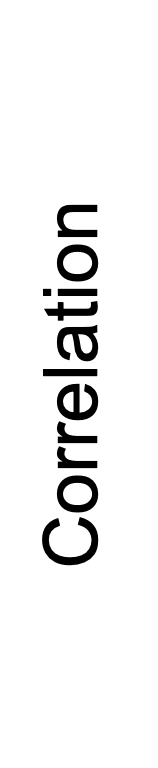
\includegraphics[scale=0.15]{figures/correlation_y_label.png}
    \end{minipage}
    \begin{minipage}{0.16\textwidth}
    \centering
    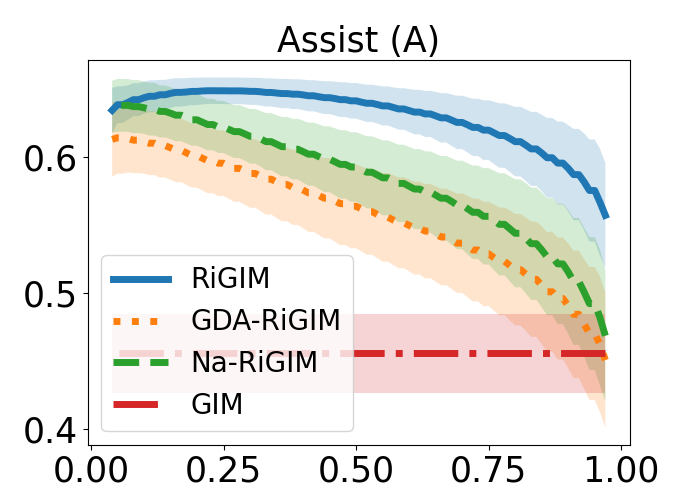
\includegraphics[scale=0.17]{figures/risk_curve_A_shadow.png}\par
    \vspace{-0.05in}
    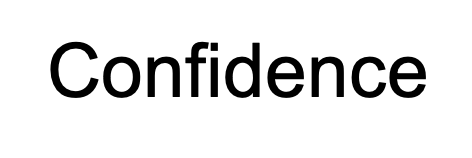
\includegraphics[scale=0.15]{figures/confidence_x_label.png}
    \end{minipage}
    \begin{minipage}{0.16\textwidth}
    \centering
    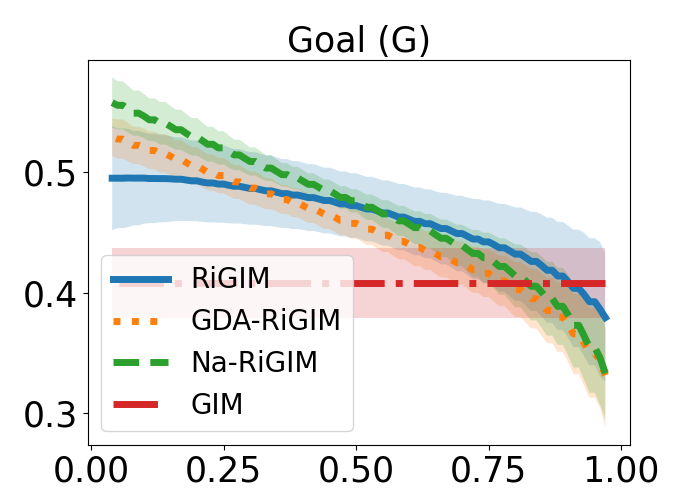
\includegraphics[scale=0.17]{figures/risk_curve_G_shadow.png}\par
    \vspace{-0.05in}
    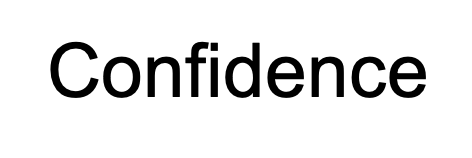
\includegraphics[scale=0.15]{figures/confidence_x_label.png}
    \end{minipage}
    \begin{minipage}{0.16\textwidth}
    \centering
    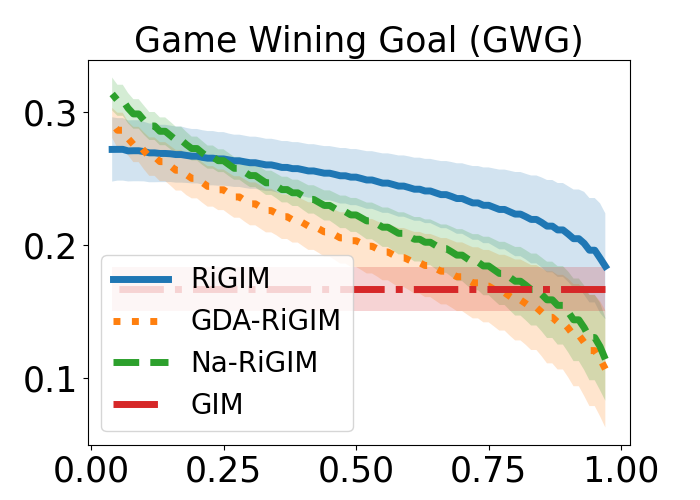
\includegraphics[scale=0.17]{figures/risk_curve_GWG_shadow.png}\par
    \vspace{-0.05in}
    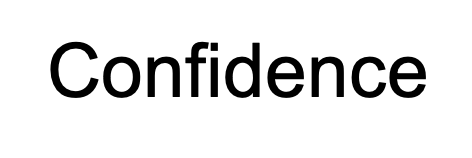
\includegraphics[scale=0.15]{figures/confidence_x_label.png}
    \end{minipage}
    \begin{minipage}{0.16\textwidth}
    \centering
    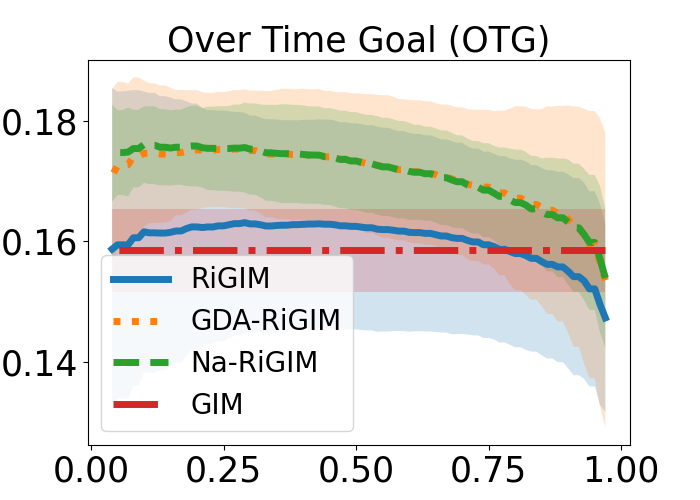
\includegraphics[scale=0.17]{figures/risk_curve_OTG_shadow.png}\par
    \vspace{-0.05in}
    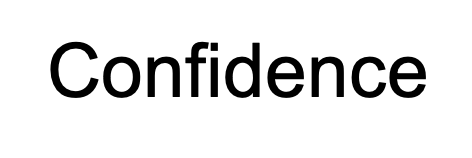
\includegraphics[scale=0.15]{figures/confidence_x_label.png}
    \end{minipage}
    \begin{minipage}{0.16\textwidth}
    \centering
    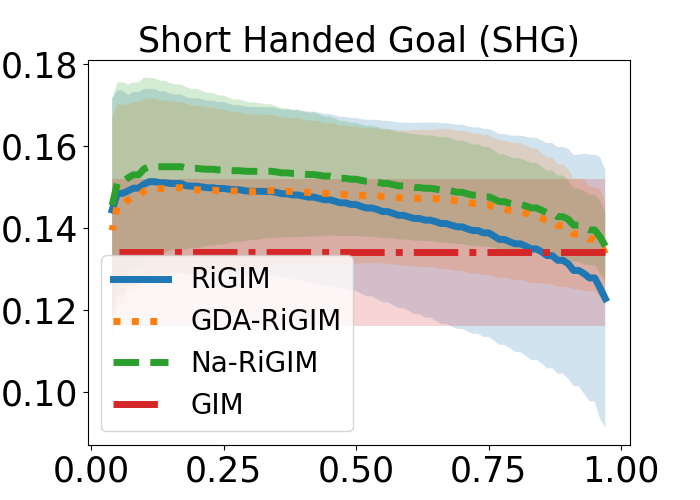
\includegraphics[scale=0.17]{figures/risk_curve_SHG_shadow.png}\par
    \vspace{-0.05in}
    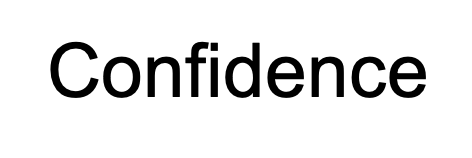
\includegraphics[scale=0.15]{figures/confidence_x_label.png}
    \end{minipage}
    \begin{minipage}{0.16\textwidth}
    \centering
    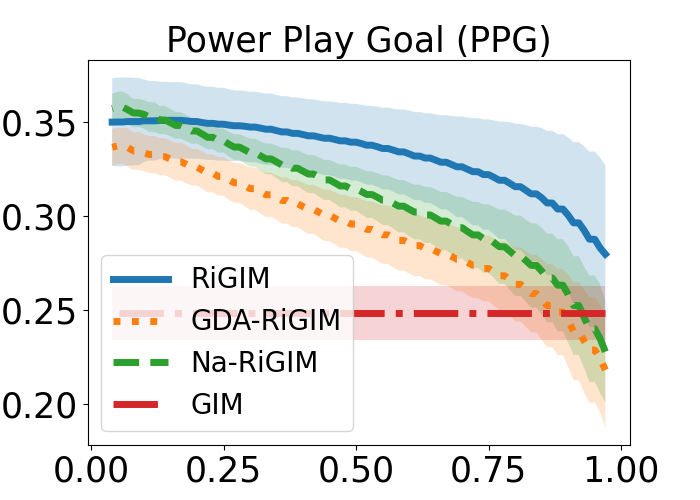
\includegraphics[scale=0.17]{figures/risk_curve_PPG_shadow.png}\par
    \vspace{-0.05in}
    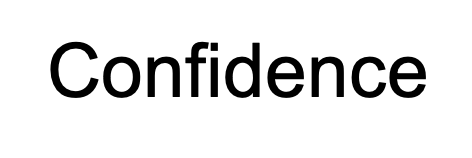
\includegraphics[scale=0.15]{figures/confidence_x_label.png}
    \end{minipage}
    \begin{minipage}{0.015\textwidth}
    \centering
    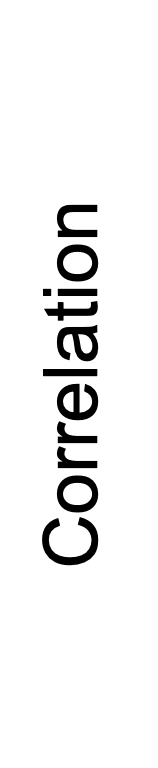
\includegraphics[scale=0.15]{figures/correlation_y_label.png}
    \end{minipage}
    \begin{minipage}{0.16\textwidth}
    \centering
    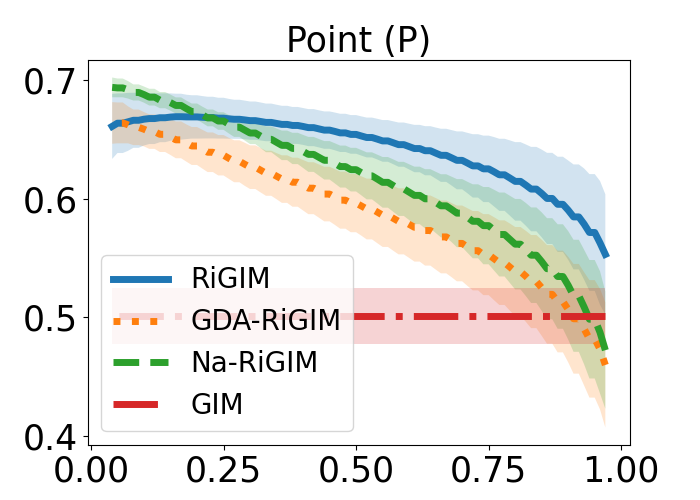
\includegraphics[scale=0.17]{figures/risk_curve_P_shadow.png}\par
    \vspace{-0.05in}
    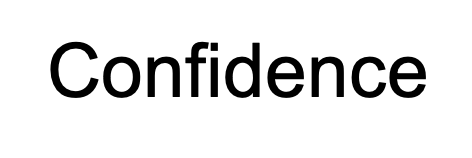
\includegraphics[scale=0.15]{figures/confidence_x_label.png}
    \end{minipage}
    \begin{minipage}{0.16\textwidth}
    \centering
    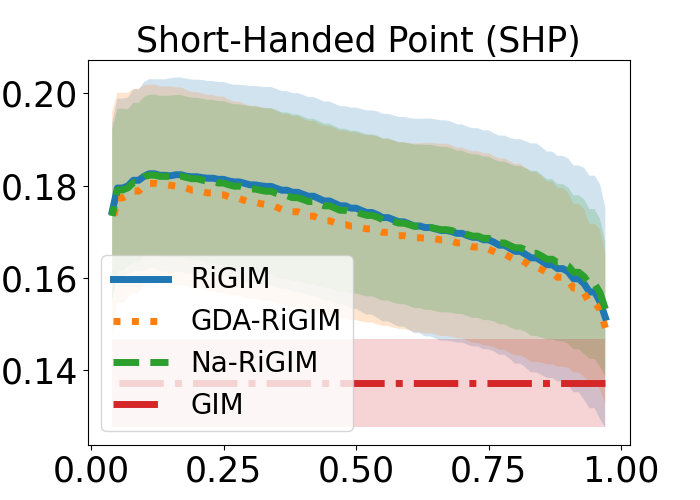
\includegraphics[scale=0.17]{figures/risk_curve_SHP_shadow.png}\par
    \vspace{-0.05in}
    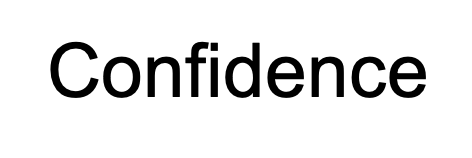
\includegraphics[scale=0.15]{figures/confidence_x_label.png}
    \end{minipage}
    \begin{minipage}{0.16\textwidth}
    \centering
    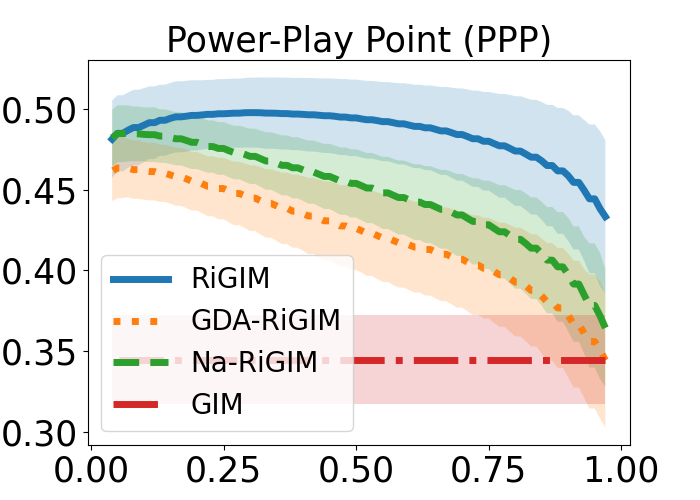
\includegraphics[scale=0.17]{figures/risk_curve_PPP_shadow.png}\par
    \vspace{-0.05in}
    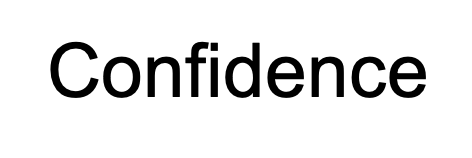
\includegraphics[scale=0.15]{figures/confidence_x_label.png}
    \end{minipage}
    \begin{minipage}{0.16\textwidth}
    \centering
    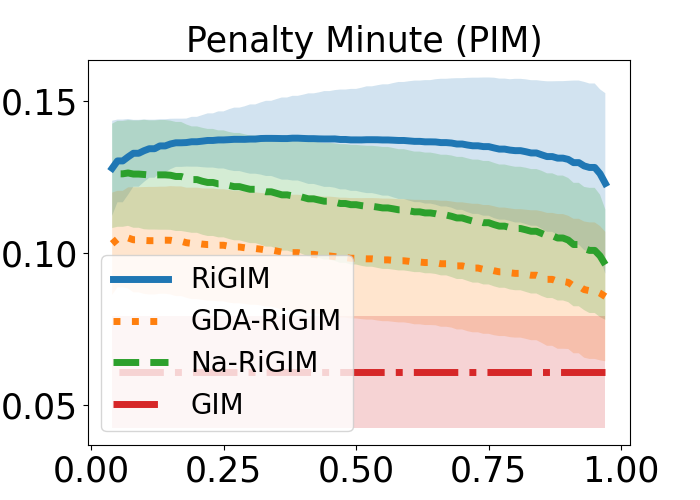
\includegraphics[scale=0.17]{figures/risk_curve_PIM_shadow.png}\par
    \vspace{-0.05in}
    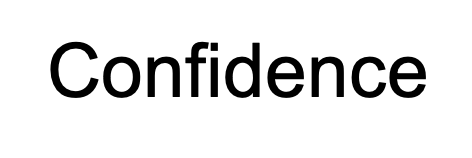
\includegraphics[scale=0.15]{figures/confidence_x_label.png}
    \end{minipage}
    \begin{minipage}{0.16\textwidth}
    \centering
    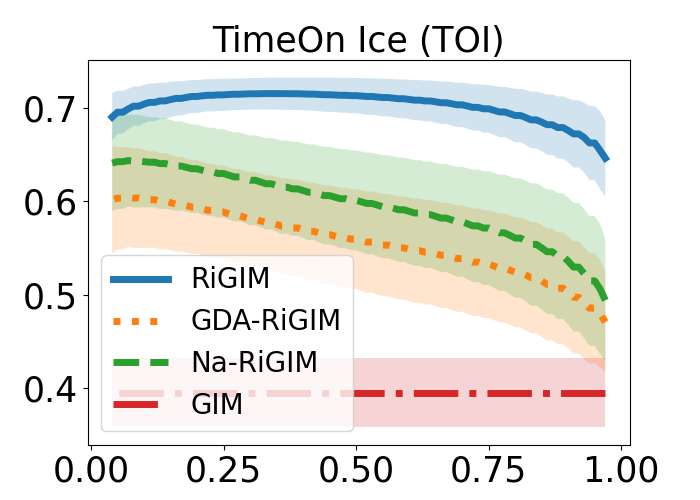
\includegraphics[scale=0.17]{figures/risk_curve_GP_shadow.png}\par
    \vspace{-0.05in}
    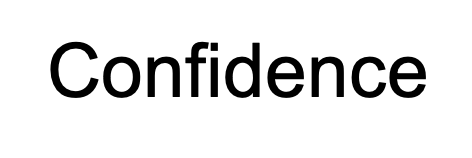
\includegraphics[scale=0.15]{figures/confidence_x_label.png}
    \end{minipage}
    \begin{minipage}{0.16\textwidth}
    \centering
    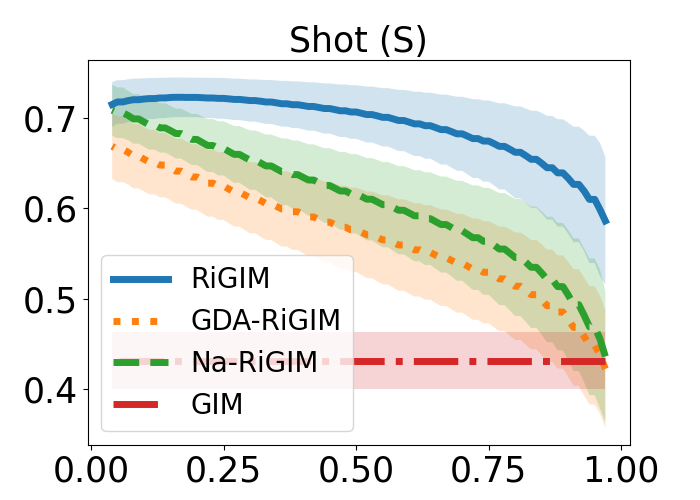
\includegraphics[scale=0.17]{figures/risk_curve_S_shadow.png}\par
    \vspace{-0.05in}
    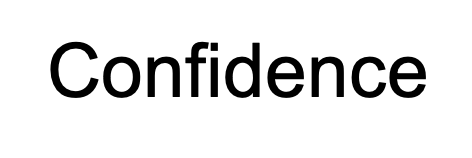
\includegraphics[scale=0.15]{figures/confidence_x_label.png}
    \end{minipage}
    % \par
    % \begin{center}
    % \vspace{-0.05in}
    % 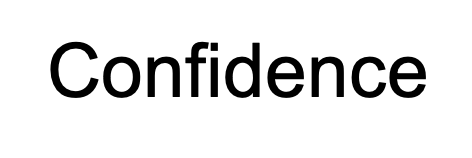
\includegraphics[scale=0.15]{figures/confidence_x_label.png}
    % \end{center}
    \vspace{-0.15in}
    \caption{Correlations (Mean $\pm$ standard deviation) between metrics and success measures at different confidence levels.}
    \vspace{-0.05in}
    \label{fig:risk-sensitivity}
\end{figure*}

\subsection{Sensitivity to Risk: Correlations Conditioning on Different Confidence Levels}
\sys$(c)$ indicates with probability $\confidence$ that the players' impact should be at least \sys$(\confidence)$.
We study whether the \sys-based metrics are sensitive to risk by 1) varying the confidence level $\confidence$ from 0 to 1 and 2) computing the correlations between the standard success measures and the metrics conditioning on $\confidence$, for example, 

Figure~\ref{fig:risk-sensitivity} shows correlations at different confidence levels. The \sys-based metrics are sensitive to risk, in the sense that their correlations change with the confidence levels, whereas GIM, as a risk-neutral metric, is unaware of the risk, and thus its correlations remain unchanged. 
Compared to other baselines, our \system generally maintains higher correlations with success measures, especially when $\confidence$ increases to 1. The exceptions are the correlations with the SHP, SHG, and OTG, which are rare events with small densities, and thus CMAF may filter them. 
We find when $\confidence$ is small, \sys$(\confidence)$ becomes risk-seeking, and thus achieves a higher correlation with success measures.
\system achieves the highest correlations when $\confidence$ is around 0.2 (as opposed to 0 for Na-\system and GDA-\system). This phenomenon is more consistent with the fact that an overly risk-seeking estimate (when $\confidence$ is 0) does not reflect the real contributions of players.



% \subsection{The Accuracy of Actions-Values: An Monte- Carlo Experiment over Game Context}
\subsection{The Prediction Accuracy: Match Future Scoring Frequencies With Action-Values}
We study how well the predicted action-value distributions match the observed next-goal scoring frequencies under discrete game contexts in the testing dataset. 
These game contexts are constructed by dividing the continuous state space into discrete bins. To calculate the empirical scoring frequency associated with each bin, we assign an observed state $\state$ to a bin $\bin$ according to the values of three discrete context features in the last observation: Manpower Differential, Goal Differential, and Period. The empirical and estimated scoring probabilities for a bin (with size $|\bin|$) are defined as follows:

a){ \it Empirical Scoring Probabilities}: for each $\state\in\bin$, we set $\goal_{\agentIndex}{(\state)} = 1$ if the observed scoring-episode containing state $\state$ ends with a goal by team $\agentIndex$. Then $\MakeUppercase{\goal}^{*}_{\agentIndex}(\bin) = \frac{1}{|\bin|}\sum_{\state \in \bin} \goal_{\agentIndex}(\state)$.

b){ \it Estimated Scoring Probabilities}: for each $\state\in\bin$, we average the $N$ samples from the calibrated distribution $z_{\agentIndex}(\state)\sim\hat{Z}_{\agentIndex}(\state,\action)\mathbb{I}_{p(\cdot|\condition)\geq\epsilon}$ to compute the estimated scoring probabilities : $\hat{\MakeUppercase{\goal}}_{\agentIndex}(\bin) = \frac{1}{N|\bin|}\sum_{\state \in \bin} \sum_{n=1}^{N}z_{\agentIndex,n}(\state)$.



% \begin{table*}[htbp]
% \setlength{\tabcolsep}{4pt}
% % \setlength\extrarowheight{5pt}
% \centering
% \resizebox{1\textwidth}{!}{
% \begin{tabular}{l|ccc|ccc|ccc}
% \toprule
% \multirow{2}{*}{Context} & \multicolumn{3}{|c}{Manpower Differential} & \multicolumn{3}{|c}{Score Difference} & \multicolumn{3}{|c}{Period}\\ \cline{2-10} 
%  & Short-Handed & Even-Strength & Power-Play & -1 & 0 & 1 & Third & Second & First \\ \hline
% GIM & 0.115 $\pm$ 0.078 & 0.094 $\pm$ 0.082 & 0.099 $\pm$ 0.085 & 0.238 $\pm$ 0.122 & 0.105 $\pm$ 0.084 & 0.271 $\pm$ 0.059 & 0.095 $\pm$ 0.055 & 0.111 $\pm$ 0.086 & 0.114 $\pm$ 0.084 \\
% Na-RiGIM &  &  &  &  &  & \\
% GDA-RiGIM & 0.148 & 0.072 & 0.017 & 0.236 & 0.045 & 0.110 & 0.143 & 0.05 & 0.033 \\
% RiGIM &  &  &  &  &  &  \\ \bottomrule
% \end{tabular}
% }
% \end{table*}
% \vspace{-0.1in}
\begin{table}[htbp]
\centering
\resizebox{0.5\textwidth}{!}{
\begin{tabular}{l|ccc}
\toprule
\begin{tabular}[c]{@{}c@{}}Manpower\\ Differential\end{tabular}& \begin{tabular}[c]{@{}c@{}}Short-\\ Handed\end{tabular} & \begin{tabular}[c]{@{}c@{}}Power-\\ Play\end{tabular} & \begin{tabular}[c]{@{}c@{}}Power-\\ Play\end{tabular}  \\\hline
% GIM(T1) &  &  &  \\
GIM & 0.115 $\pm$ 0.078 & 0.094 $\pm$ 0.082 & 0.099 $\pm$ 0.085  \\
Na-RiGIM & 0.133 $\pm$ 0.016 & 0.064 $\pm$ 0.016 & {\bf 0.013} $\pm$ 0.009 \\
GDA-RiGIM & 0.148 $\pm$ 0.035 & 0.072 $\pm$ 0.029 & 0.017 $\pm$ 0.011  \\
RiGIM & {\bf 0.080} $\pm$ 0.020 & {\bf 0.058} $\pm$ 0.008 & 0.047 $\pm$ 0.046 \\ \hline\hline
% \end{tabular}
% }
% \end{table}
% \begin{table}[htbp]
% \centering
% \resizebox{0.45\textwidth}{!}{
% \begin{tabular}{l|ccc}
% \toprule
 Goal Differential & -1 & 0 & 1 \\\hline
% GIM(T1) &  &  &  \\
GIM  & 0.238 $\pm$ 0.122 & 0.105 $\pm$ 0.084 & 0.271 $\pm$ 0.059 \\
Na-RiGIM  & 0.238 $\pm$ 0.006 & 0.045 $\pm$ 0.015 & 0.108 $\pm$ 0.031 \\
GDA-RiGIM & 0.236 $\pm$ 0.007 & 0.045 $\pm$ 0.016 & 0.11 $\pm$ 0.027 \\
RiGIM & {\bf 0.193} $\pm$ 0.021 & {\bf 0.029} $\pm$ 0.015 & {\bf 0.092} $\pm$ 0.019 \\ \hline\hline
% \end{tabular}
% }
% \end{table}

% \begin{table}[htbp]
% \centering
% \resizebox{0.45\textwidth}{!}{
% \begin{tabular}{l|ccc}
% \toprule
Period & 3 & 2 & 1 \\\hline
% GIM(T1) &  &  &  \\
GIM & {\bf 0.095} $\pm$ 0.055 & 0.111 $\pm$ 0.086 & 0.114 $\pm$ 0.084\\
Na-RiGIM  & 0.139 $\pm$ 0.018 & 0.044 $\pm$ 0.015 & 0.024 $\pm$ 0.015 \\
GDA-RiGIM & 0.143 $\pm$ 0.028 & 0.050 $\pm$ 0.025 & 0.033 $\pm$ 0.025  \\
RiGIM & 0.143 $\pm$ 0.011 & {\bf 0.032} $\pm$ 0.005 & {\bf 0.014} $\pm$ 0.009 \\ \bottomrule
\end{tabular}
}
\vspace{-0.1in}
\caption{The absolute difference between the empirical and the estimated Scoring Probabilities for a total of 9 bins.}
\label{table:calibration-results}
% \vspace{-0.1in}
\end{table}

Table~\ref{table:calibration-results} shows the average absolute difference between $\hat{\MakeUppercase{\goal}}$ and $\MakeUppercase{\goal}^{*}$ based on 5 independent runs. To derive a fair comparison, baselines mainly contain the learning-based action-values functions for the context-aware player evaluation. \system achieves a minimum distance in 7 out of 9 bins. This is because 1) MAF outperforms GDA by developing a more accurate uncertainty estimator for filtering OoD states and 2) the distribution estimates contain a richer information (e.g., multi-modality) than expectation estimate, allowing $\Tilde{Z}(\cdot)$ to better match the scoring frequencies than $Q(\cdot)$. This obervation is consistent with the findings in \cite{bellemare2017distributional}.

\section{Conclusion and Future Work}

In this paper, we designed an RL framework for quantifying the aleatoric uncertainty and the epistemic uncertainty from a play-by-play ice hockey dataset. This framework enabled distributional RL and a MAF model to estimate both uncertainties, with which we proposed a risk-sensitive evaluation metric \system. Empirical results showed \system correlated well with success measures and the correlation is sensitive to confidence levels. For future works, we will develop a soft calibration method that can adjust the distributions for OoD samples and scale our method to other professional sports.

\textcolor{blue}{Don't forget to acknowledge NSERC and sportlogiq}

\newpage
\section*{Ethics Statement}
We expect the main impact outside of the machine learning community to be in professional sports. As an entertainment industry, professional sports increase the quality of life for many people. Fans, media, and clubs can be better engaged in sports games with a player ranking system, but putting players’ performance under intense scrutiny may yield more pressure on the professional players. The overwhelming pressure might cause anxiety and thus contradicts the original purpose of evaluating players, which is about improving their playing skills and market value.


\bibliographystyle{named}
\bibliography{bibliography.bib}



\end{document}

